% =====================================================================================
%  flow_matching_safe_set_POC.tex
%
%  Proof of concept: order-1 Wasserstein conformal safe sets for time-dependent vector
%  fields (diffusion models and linear flow matching).  Self-contained folder:
%  custom_2020.sty, informs2014.bst and refs.bib are copied here; figures/ and tables/
%  are generated from results/ by code/make_figures.py and code/make_tables.py.
%  Build (from this folder):
%      pdflatex flow_matching_safe_set_POC && bibtex flow_matching_safe_set_POC
%      && pdflatex flow_matching_safe_set_POC && pdflatex flow_matching_safe_set_POC
%  Every number in the experimental section is read from tables/numbers.tex and the
%  tables/*.tex bodies, written by code/make_tables.py (see Appendix A).
% =====================================================================================
\documentclass{article}
\usepackage[preprint]{custom_2020}
\usepackage{amsmath}
\usepackage{stmaryrd}
\usepackage{tgtermes}
\usepackage[dvipsnames]{xcolor}
\usepackage{bm}
\usepackage{dsfont}
\usepackage{bbm}
\usepackage{mathrsfs}
\usepackage[hidelinks]{hyperref}
\usepackage{amssymb,amsfonts}
\usepackage{caption}
\usepackage{subcaption}
\usepackage{graphicx}
\usepackage{url}
\usepackage{booktabs}
\usepackage{array}
\usepackage{tabularx}
\usepackage{multirow}
\usepackage{mathtools}
\usepackage{algorithm}
\usepackage{algpseudocode}
\usepackage[section]{placeins}   % floats stay inside their section

% ---------- operators (as in main.tex) ----------
\DeclareMathOperator*{\argmin}{arg\,min}
\DeclareMathOperator{\E}{\mathbb{E}}
\DeclareMathOperator{\card}{card}
\DeclareMathOperator{\conv}{conv}
\DeclareMathOperator{\quantile}{Quantile}
\DeclareMathOperator{\tr}{tr}
\DeclareMathOperator{\dist}{dist}
\DeclareMathOperator{\vect}{vec}
\newcommand{\RR}{\mathbb{R}}
\newcommand{\NN}{\mathbb{N}}

% ---------- notation of this note ----------
\newcommand{\cV}{\mathcal{V}}                       % space of fields
\newcommand{\cD}{\mathcal{D}}                       % training (historical) fields
\newcommand{\Pv}[1]{P^{#1}}                         % path law of the chain driven by a field
\newcommand{\Pbar}{\bar{P}}                         % mixture of historical path laws
\newcommand{\TV}{\mathrm{TV}}
\newcommand{\KL}{\mathrm{KL}}
\newcommand{\kl}{\mathrm{kl}}
\newcommand{\klinv}{\mathrm{kl}^{-1}}
\newcommand{\Sc}{S_c}                               % order-1 score with cost c
\newcommand{\Gon}{G_{\mathrm{on}}}
\newcommand{\GKL}{G_{\mathrm{KL}}}
\newcommand{\bth}{\boldsymbol{\theta}}
\newcommand{\bx}{\mathbf{x}}
\newcommand{\by}{\mathbf{y}}
\newcommand{\bz}{\mathbf{z}}
\newcommand{\bxi}{\boldsymbol{\xi}}
\newcommand{\be}{\mathbf{e}}                       % prompt embedding

\usepackage{natbib}
 \bibpunct[, ]{(}{)}{,}{a}{}{,}%
 \def\bibfont{\small}%
 \def\bibsep{\smallskipamount}%
 \def\bibhang{24pt}%
 \def\newblock{\ }%
 \def\BIBand{and}%

\usepackage{amsthm}
\theoremstyle{plain}
\newtheorem{theorem}{Theorem}
\newtheorem{lemma}{Lemma}
\newtheorem{definition}{Definition}
\newtheorem{corollary}{Corollary}
\newtheorem{proposition}{Proposition}
\newtheorem{remark}{Remark}
\newtheorem{assumption}{Assumption}

\newcommand{\pairKLAmed}{0.067}
\newcommand{\pairKLAninety}{0.257}
\newcommand{\pALmean}{8.3\times 10^{-6}}
\newcommand{\pairKLDmed}{0.378}
\newcommand{\pairKLDninety}{0.755}
\newcommand{\pALDmean}{0.0004}
\newcommand{\pALCmean}{0.0017}
\newcommand{\covAF}{0.897}
\newcommand{\covAK}{0.898}
\newcommand{\exclAFthree}{0.42}
\newcommand{\exclAKthree}{1.00}
\newcommand{\exclAKone}{0.83}
\newcommand{\exclAFone}{0.19}
\newcommand{\exclCrefthree}{0.15}
\newcommand{\exclConthree}{0.55}
\newcommand{\exclDfwdthree}{0.17}
\newcommand{\exclDrevthree}{0.55}
\newcommand{\exclDfwdten}{0.69}
\newcommand{\exclCononeP}{0.133}
\newcommand{\exclConthreeP}{0.552}
\newcommand{\exclDrevoneP}{0.129}
\newcommand{\exclDrevthreeP}{0.546}
\newcommand{\certAKmed}{0.031}
\newcommand{\certAFmed}{0.283}
\newcommand{\certDrevmed}{0.134}
\newcommand{\certDfwdmed}{0.553}
\newcommand{\insideAKmed}{0.0123}
\newcommand{\insideAFmed}{0.0324}
\newcommand{\insideAFmax}{0.0947}
\newcommand{\insideDrevmed}{0.0145}
\newcommand{\insideDfwdmed}{0.0707}
\newcommand{\geoCrefclean}{0.28}
\newcommand{\geoConclean}{0.35}
\newcommand{\winCrefclean}{32}
\newcommand{\winConclean}{32}
\newcommand{\geoCrefcont}{0.21}
\newcommand{\geoConcont}{0.20}
\newcommand{\winCrefcont}{32}
\newcommand{\winConcont}{32}
\newcommand{\ntasks}{32}
\newcommand{\pAUcont}{0.138}
\newcommand{\pACrefcont}{0.047}
\newcommand{\pAConcont}{0.025}
\newcommand{\pASten}{0.0087}
\newcommand{\backoffmax}{0.011}
\newcommand{\backofffrac}{0.70}
\newcommand{\socptime}{0.31}
\newcommand{\epsref}{0.0182}
\newcommand{\epson}{0.0193}
\newcommand{\exampletask}{8}
\newcommand{\exUpA}{0.133}
\newcommand{\exCrefpA}{0.029}
\newcommand{\exConpA}{0.013}
\newcommand{\exSpA}{0.009}
\newcommand{\excentrepA}{0.001}
\newcommand{\exoraclepA}{0.003}
\newcommand{\excentresref}{0.55}
\newcommand{\excentreson}{0.54}
\newcommand{\lipmin}{52}
\newcommand{\lipmax}{53}
\newcommand{\gronwalllog}{15}

% primitive (expandable) input, so that table bodies can be read inside tabular
\makeatletter\newcommand{\inputrows}[1]{\@@input #1 }\makeatother

\title{Conformal safe sets for time-dependent vector fields:\\[3pt]
\large the order-$1$ Wasserstein score for diffusion models and linear flow matching
(proof of concept)}
\author{Companion note to \emph{Pipeline-Agnostic Meta-Learning: an Optimal Transport
Approach}}
\date{\today}

\begin{document}
\maketitle

\begin{abstract}
The manuscript constrains a new model to the order-$1$ Wasserstein conformal region built
from historical model weights. This note extends the construction from weight vectors to the
time-dependent vector fields that drive diffusion and flow-matching models, so that a newly
trained field is kept close to historical \emph{safe} fields. The closed form of the order-$1$
score holds on any pseudometric space (Lemma~\ref{lem:closed_form}), and split-conformal
coverage holds for any cost (Proposition~\ref{pr:coverage}); the open question is which cost
encodes safety. Viewing samplers as Gaussian-increment chains makes the path divergence
between two samplers an explicit time-weighted integral of the squared field difference
(Lemma~\ref{lem:chain_kl}). With this cost, every field of the region inherits the safety of the
historical mixture, in total variation (Theorem~\ref{th:tv}) and, for the reverse divergence, in
the sense that events that are rare under the safe samplers stay rare (Theorem~\ref{th:rare}).
The direction matters: a forward cost charges at most $\log(1/(1-m))$ for an unsafe mode of
mass $m$, the reverse cost about $m\log(m/q)$, where $q$ is the safe probability of the unsafe
region (Proposition~\ref{pr:direction}). For a flow-matching velocity that is linear in its
parameters, the field distance is a Mahalanobis distance whose Gram matrix is the average of the
historical least-squares Gram matrices; after whitening the region is the Euclidean region of the
manuscript and constrained training is a second-order cone program
(Propositions~\ref{pr:mahalanobis}--\ref{pr:socp}). A two-dimensional toy experiment checks the
coverage, the forward/reverse gap, the certificates on $200$ random splits, and constrained
few-shot fine-tuning against least squares and shrinkage. For prompt-conditioned models, where safe prompts induce
safe fields, time collapses for straight flows (the field is constant along trajectories), the
distance between noise-to-output maps carries a Wasserstein certificate without Gr\"onwall
factor, and forcing a prompt into the safe set has closed forms. A catalogue of design choices
and an experiment plan close the note.
\end{abstract}

\setcounter{tocdepth}{1}
\tableofcontents

% =====================================================================================
\section{Introduction}\label{sec:intro}
% =====================================================================================

In the manuscript, a deterministic pipeline $f$ maps a task to a weight vector
$\bth\in\Theta\subseteq\RR^d$. The historical weights $\bth_1,\dots,\bth_M$ define the
order-$1$ nonconformity score
\begin{equation}\label{eq:manuscript_score}
  s_{d,1}(\bth;\cD)=\frac{1}{M(M+1)}\sum_{i=1}^M d(\bth,\bth_i)
  =W_{d,1}\Big(\hat{\mathbbm{F}}_M,\tfrac{1}{M+1}\big(M\hat{\mathbbm{F}}_M+\delta_{\bth}\big)\Big),
\end{equation}
and split conformal prediction turns a calibration set into a radius $\varepsilon$ such that
the region $\{\bth:s_{d,1}(\bth;\cD)\leq\varepsilon\}$ contains the pipeline's output for a
new task with probability at least $1-\beta$. Training on a new task is then restricted to
this region (problem \texttt{OT1-TRAIN} in the manuscript).

Diffusion models \citep{ho2020denoising,song2021score} and flow-matching models
\citep{lipman2023flow,liu2023flow,albergo2023building} are not described by a weight
vector at sampling time but by a \emph{time-dependent vector field}: a score field
$s(\bx,t)$ or a velocity field $v(\bx,t)$, integrated by a sampler from noise to data.
Diffusion policies \citep{chi2023diffusion} use the same object to generate control
actions. The question addressed here is whether the order-$1$ region can be built on the
space of such fields, so that a field trained on a new task (possibly with few or
corrupted samples) is forced to stay close to historical fields that are known to be safe.

\paragraph{What carries over and what has to be chosen.}
Lemma~\ref{lem:closed_form} shows that the closed form \eqref{eq:manuscript_score} only
uses the triangle inequality, so it holds for any pseudometric on fields.
Proposition~\ref{pr:coverage} recalls that split-conformal coverage does not even need a
metric: any cost that is fixed once the training fields are fixed gives a valid region. The
substantive choice is therefore the cost $c(v,v_i)$ between a candidate field and a
historical field. Section~\ref{sec:chains} shows that the samplers used in practice are
Gaussian-increment Markov chains, for which the Kullback--Leibler divergence between the
path laws of two samplers is an explicit, time-weighted integral of the squared field
difference (Lemma~\ref{lem:chain_kl}). This answers the question of how to handle time: the
weight given to each time step is dictated by the sampler and is not a free choice.

\paragraph{Safety semantics.}
Section~\ref{sec:safety} shows what membership in the region implies. With a cost that
upper-bounds the total variation, every field in the region generates trajectories whose
law is within an explicit total-variation distance of the mixture of the historical
samplers (Theorem~\ref{th:tv}). With the \emph{reverse} Kullback--Leibler divergence, measured
along the candidate's own trajectories, the guarantee is of a different nature: any event
that is rare under the historical safe samplers remains rare
(Theorem~\ref{th:rare}). Proposition~\ref{pr:direction} explains why the direction
matters, and the experiments confirm it: forward costs, which are convex and cheap, let
through fields that place a few percent of their mass in an unsafe region; reverse costs do
not. None of these results requires the unsafe event to be known: they hold for every
event simultaneously.

\paragraph{Linear flow matching.}
Section~\ref{sec:linear} treats velocity fields that are linear in their parameters,
$v_{\bth}(\bx,t)=\Phi(\bx,t)\bth$. Historical fits are least squares. The $L^2$ distance between
two fields is a Mahalanobis distance on the parameters, and its Gram matrix under the
pooled interpolation path is the average of the historical least-squares Gram matrices
(Proposition~\ref{pr:mahalanobis}). After whitening, the region is the Euclidean order-$1$
region of the manuscript, so the existing machinery (geometric median, task reweighting,
gauge parametrisation) applies unchanged and \texttt{OT1-TRAIN} becomes a second-order cone
program (Proposition~\ref{pr:socp}). The same linear model can be sampled with a stochastic
differential equation that has the same marginals (Lemma~\ref{lem:sde}); the path divergence is
then a quadratic form in the parameters with a Gram matrix measured along the candidate's
own trajectories (Corollary~\ref{cor:fm_kl}).

\paragraph{Prompt-conditioned models.}
Section~\ref{sec:prompts} specialises the construction to a trained flow-matching model conditioned on
prompt embeddings, where a collection of safe prompts defines a collection of safe fields. For a
straight flow the velocity is constant along each trajectory, so the time-dependent field is
summarised by its slice at $t=0$ (Lemma~\ref{lem:straight}); flows trained with the linear
interpolant are not straight in general (Remark~\ref{rem:not_straight}). Comparing the noise-to-output
maps of two prompts under shared noise gives a Wasserstein certificate without the Gr\"onwall factor
of Proposition~\ref{pr:ode} (Theorem~\ref{th:map_cert}), and forcing a prompt into the safe set has
closed forms: one-step blending (Proposition~\ref{pr:blend}) and, for a model affine in the prompt, a
projection of the prompt embedding (Proposition~\ref{pr:prompt_proj}). Section~\ref{sec:catalogue}
catalogues the costs, regions, enforcement mechanisms and calibration procedures that the analysis
supports, and Section~\ref{sec:plan} proposes experiments to test them.

\paragraph{Experiments.}
Section~\ref{sec:experiments} reports a two-dimensional proof of concept: tasks are rotated
and rescaled four-blob rings, and the unsafe set is a disk at the centre that no task
visits. Coverage is within sampling error of the nominal level for every cost. The reverse
costs exclude contaminated fields that the forward costs admit. The certificates hold on all
$200$ random splits, and the reverse-KL certificate is about nine times tighter than the
total-variation one with exact scores, and four times with linear fits. Constrained few-shot fine-tuning improves markedly on least squares,
but in this concentrated task family it is beaten by strong shrinkage towards the centre of
the region. Section~\ref{sec:discussion} lists the limitations.

% =====================================================================================
\section{Setting and notation}\label{sec:setting}
% =====================================================================================

\paragraph{Tasks, pipelines and fields.}
Tasks $\tau$ are drawn from a meta-distribution $\mathbbm{Q}$. A pipeline $f$ maps a task to
an element $v=f(\tau)$ of a set $\cV$ of \emph{fields}. In this note a field is a
time-dependent vector field $v:\RR^n\times[0,1]\to\RR^n$ (flow matching) or a score field
$s:\RR^n\times(0,T]\to\RR^n$ (diffusion); when fields are parametrised, $\cV$ can be
identified with the parameter space. The pipeline may use internal randomness (finite data,
Monte Carlo); it is applied independently to each task. We write
$\cD=(v_1,\dots,v_M)$ for the \emph{training} (historical) fields,
$v_{M+1},\dots,v_{M+K}$ for the \emph{calibration} fields and $v_{M+K+1}$ for the field of a
new task.

\paragraph{Order-$1$ score with an arbitrary cost.}
\begin{definition}[Order-$1$ score]\label{def:score}
Let $c:\cV\times\cV\to[0,+\infty]$ be measurable (not necessarily symmetric, not necessarily
satisfying the triangle inequality), let $\cD=(v_1,\dots,v_M)$ and let $w$ be a probability
vector on $\llbracket M\rrbracket$. The weighted order-$1$ score of $v\in\cV$ is
\begin{equation}\label{eq:score}
  S^w_c(v;\cD)\coloneqq\frac{1}{M+1}\sum_{i=1}^M w_i\,c(v,v_i),
  \qquad
  S_c(v;\cD)\coloneqq S^{(1/M,\dots,1/M)}_c(v;\cD)=\frac{1}{M(M+1)}\sum_{i=1}^M c(v,v_i).
\end{equation}
\end{definition}
For $c=d$ a metric on weights, $S_c$ is the score $s_{d,1}$ of \eqref{eq:manuscript_score} and
$S^w_c$ is the task-adaptive score $g_{d,1}$ of the manuscript. Note that
\begin{equation}\label{eq:budget}
  S^w_c(v;\cD)\leq\varepsilon
  \quad\Longleftrightarrow\quad
  \sum_{i=1}^M w_i\,c(v,v_i)\leq(M+1)\,\varepsilon .
\end{equation}
The quantity $(M+1)\varepsilon$ is therefore the budget on the $w$-average cost, and it is
the quantity that appears in all safety statements below.

\begin{definition}[Split-conformal threshold and region]\label{def:region}
Let $\beta\in(0,1)$, $k\coloneqq\lceil(K+1)(1-\beta)\rceil$, and let $S_j\coloneqq\Sc(v_{M+j};\cD)$,
$j\in\llbracket K\rrbracket$, be the calibration scores. The threshold $\varepsilon$ is the
$k$-th smallest of $S_1,\dots,S_K$ if $k\leq K$ and $+\infty$ otherwise; this is
$C_{1-\beta}(S_1,\dots,S_K)$ in the notation of the manuscript. The region is
$\bar{\cV}\coloneqq\{v\in\cV:\Sc(v;\cD)\leq\varepsilon\}$.
\end{definition}

\paragraph{Probability metrics.}
For probability measures $P,Q$ on a common measurable space,
$\TV(P,Q)\coloneqq\sup_A|P(A)-Q(A)|$ (supremum over measurable sets),
$\KL(P\|Q)\coloneqq\E_P[\log\tfrac{dP}{dQ}]$ if $P\ll Q$ and $+\infty$ otherwise, and for
$p,q\in[0,1]$ the binary divergence is
$\kl(p\|q)\coloneqq p\log\tfrac{p}{q}+(1-p)\log\tfrac{1-p}{1-q}$ with $0\log0=0$.

% =====================================================================================
\section{The order-1 score on a space of fields}\label{sec:score}
% =====================================================================================

\begin{lemma}[Closed form on a pseudometric space]\label{lem:closed_form}
Let $(\cV,d)$ be a pseudometric space: $d\geq0$ is symmetric, satisfies the triangle
inequality and $d(v,v)=0$ (distinct points may be at distance zero). Let
$v_1,\dots,v_M,v\in\cV$, let $w$ be a probability vector on $\llbracket M\rrbracket$, and set
\[
  \mu_w\coloneqq\sum_{i=1}^M w_i\,\delta_{v_i},
  \qquad
  \nu_w\coloneqq\frac{M}{M+1}\,\mu_w+\frac{1}{M+1}\,\delta_{v}.
\]
Let $W_{d,1}(\mu,\nu)\coloneqq\min_{\pi\in\Pi(\mu,\nu)}\int d\,d\pi$, where $\Pi(\mu,\nu)$ is the
set of couplings of the two finitely supported measures. Then
\[
  W_{d,1}(\mu_w,\nu_w)=\frac{1}{M+1}\sum_{i=1}^M w_i\,d(v_i,v)=S^w_d(v;\cD).
\]
In particular, for $w_i=1/M$, $W_{d,1}(\hat{\mathbbm{F}}_M,\frac{1}{M+1}(M\hat{\mathbbm{F}}_M+\delta_v))=\frac{1}{M(M+1)}\sum_i d(v_i,v)$.
\end{lemma}
\textit{Proof:}
\emph{Step 1 (a feasible plan: the upper bound).} Let
$\pi^\star\coloneqq\sum_i\frac{Mw_i}{M+1}\delta_{(v_i,v_i)}+\sum_i\frac{w_i}{M+1}\delta_{(v_i,v)}$.
Its first marginal is $\sum_i w_i\delta_{v_i}=\mu_w$ and its second marginal is
$\frac{M}{M+1}\mu_w+\frac{1}{M+1}\delta_v=\nu_w$, since $\sum_iw_i=1$. Hence
$\pi^\star\in\Pi(\mu_w,\nu_w)$ and, using $d(v_i,v_i)=0$,
$W_{d,1}(\mu_w,\nu_w)\leq\int d\,d\pi^\star=\frac{1}{M+1}\sum_iw_i\,d(v_i,v)$.

\emph{Step 2 (every plan costs at least as much: the lower bound).} Let $\pi\in\Pi(\mu_w,\nu_w)$
and let $g(x)\coloneqq d(x,v)$. The triangle inequality $d(x,v)\leq d(x,y)+d(y,v)$ gives
$d(x,y)\geq g(x)-g(y)$ for all $x,y\in\cV$. Integrating against $\pi$ and using its marginals,
\[
  \int d\,d\pi\;\geq\;\int g\,d\mu_w-\int g\,d\nu_w
  =\sum_iw_i\,d(v_i,v)-\frac{M}{M+1}\sum_iw_i\,d(v_i,v)-\frac{1}{M+1}\,d(v,v)
  =\frac{1}{M+1}\sum_iw_i\,d(v_i,v).
\]
\emph{Step 3.} Steps~1 and~2 give the equality. \hfill $\square$

\begin{remark}
Lemma~\ref{lem:closed_form} is \texttt{lem:trivial\_W1} of the manuscript (case
$w_i=1/M$, $d$ a metric on $\RR^d$), and its weighted form is equation
\texttt{eq:adaptive\_W1}. Step~2 replaces the ``intermediate destination'' argument of the
manuscript by a single application of the triangle inequality, which is why the result holds
on any pseudometric space, in particular on spaces of time-dependent fields with the
distances of Section~\ref{sec:linear}.
\end{remark}

\begin{proposition}[Coverage for an arbitrary cost]\label{pr:coverage}
Let $c$ be a cost as in Definition~\ref{def:score}, possibly depending on an auxiliary random
element $\Xi$ (for instance the noise of Monte Carlo probe trajectories), and assume that,
conditionally on $(\cD,\Xi)$, the vector $(v_{M+1},\dots,v_{M+K},v_{M+K+1})$ is exchangeable.
Let $S_j\coloneqq\Sc(v_{M+j};\cD)$ for $j\in\llbracket K+1\rrbracket$, and let $\varepsilon$ be
the threshold of Definition~\ref{def:region}. Then
\[
  \mathbbm{P}\big(\Sc(v_{M+K+1};\cD)\leq\varepsilon\,\big|\,\cD,\Xi\big)\geq\frac{k}{K+1}\geq1-\beta,
  \qquad k=\lceil(K+1)(1-\beta)\rceil .
\]
\end{proposition}
\textit{Proof:}
\emph{Step 1 (trivial case).} If $k>K$, then $\varepsilon=+\infty$ and the event has
probability one.

\emph{Step 2 (event inclusion).} Let $k\leq K$ and let $s_{[1]}\leq\dots\leq s_{[K+1]}$ be the
order statistics of all $K+1$ scores $S_1,\dots,S_{K+1}$. For $j\in\llbracket K+1\rrbracket$ let
$E_j\coloneqq\{S_j>s_{[k]}\}$. If $S_{K+1}>\varepsilon$, then the $k$ smallest calibration
scores are all strictly smaller than $S_{K+1}$; these are $k$ of the $K+1$ scores, so
$s_{[k]}\leq\varepsilon<S_{K+1}$, i.e.\ $E_{K+1}$ holds. Hence
$\{S_{K+1}>\varepsilon\}\subseteq E_{K+1}$.

\emph{Step 3 (deterministic count).} At least $k$ indices $j$ satisfy $S_j\leq s_{[k]}$, so at
most $K+1-k$ indices satisfy $E_j$: $\sum_{j=1}^{K+1}\mathbbm{1}_{E_j}\leq K+1-k$ pointwise.

\emph{Step 4 (exchangeability).} Conditionally on $(\cD,\Xi)$ the score function $\Sc(\cdot;\cD)$
is fixed, so $(S_1,\dots,S_{K+1})$ is exchangeable and $\mathbbm{P}(E_j\mid\cD,\Xi)$ does not
depend on $j$. Taking the conditional expectation of Step~3,
$(K+1)\,\mathbbm{P}(E_{K+1}\mid\cD,\Xi)\leq K+1-k$.

\emph{Step 5.} By Steps~2 and~4,
$\mathbbm{P}(S_{K+1}\leq\varepsilon\mid\cD,\Xi)\geq1-\frac{K+1-k}{K+1}=\frac{k}{K+1}\geq1-\beta$.
\hfill $\square$

\begin{remark}[What the statement does and does not say]\label{rem:coverage}
(i) The probability is conditional on the training fields (and on $\Xi$) and marginal over
the calibration fields and the new field. A statement conditional on the calibration fields
as well requires the training-conditional (PAC) form of \citet{vovk2013conditional}; this is
the same distinction as the one flagged for \texttt{cor:ot1\_cp} of the manuscript.
(ii) What is covered is the field $f(\tau)$ that the pipeline would produce on the new task
(e.g.\ with ample data), not a field fitted on few samples; restricting few-shot training to
$\bar{\cV}$ therefore excludes the pipeline's answer with probability at most $\beta$.
(iii) Exchangeability holds when tasks are i.i.d.\ and the pipeline is applied independently
to each of them. If historical safe fields are selected by an audit, the guarantee is relative
to the population of fields that pass the audit. For histories that drift over time, the
weighted conformal procedure of \citet{barber2023conformal} applies.
(iv) Monte Carlo estimates of the cost are allowed as long as their randomness is part of
$\Xi$, i.e.\ drawn once and shared by all scores (``frozen probes''): the coverage is then
exact for the estimated score. The safety implications of Section~\ref{sec:safety}, on the
other hand, are stated for the exact cost (Remark~\ref{rem:mc}).
\end{remark}

% =====================================================================================
\section{Samplers as Gaussian-increment chains}\label{sec:chains}
% =====================================================================================

\begin{definition}[Gaussian-increment chain and path law]\label{def:chain}
Fix $J\in\NN$, step sizes $h_0,\dots,h_{J-1}>0$, noise levels $\sigma_0,\dots,\sigma_{J-1}\geq0$, an
initial law $\mu_0$ on $\RR^n$ and measurable drifts $b_k:\RR^n\to\RR^n$,
$k\in\{0,\dots,J-1\}$. The chain is $X_0\sim\mu_0$ and
\[
  X_{k+1}=X_k+h_k\,b_k(X_k)+\sigma_k\,\bxi_k,\qquad k=0,\dots,J-1,
\]
with $\bxi_0,\dots,\bxi_{J-1}$ i.i.d.\ $\mathcal{N}(0,I_n)$ and independent of $X_0$. Its path law is the
law $P^b$ of $(X_0,\dots,X_J)$ on $(\RR^n)^{J+1}$. A sampler turns a field $v$ into drifts
$b[v]$; we write $\Pv{v}\coloneqq P^{b[v]}$, $P^{(i)}\coloneqq\Pv{v_i}$ for the historical fields,
and $\Pbar_w\coloneqq\sum_iw_iP^{(i)}$ for their mixture ($\Pbar\coloneqq\Pbar_{(1/M,\dots,1/M)}$).
An \emph{event} is a measurable set $A\subseteq(\RR^n)^{J+1}$; in the experiments
$A=\{\|\bx_J\|\leq r_A\}$ concerns the final sample only.
\end{definition}

The samplers used below are the following; all of them start from $\mu_0=\mathcal{N}(0,I_n)$.
\begin{itemize}
\item \emph{Diffusion (variance-preserving, unit noise rate).} The forward process
$d\bx=-\tfrac12\bx\,dt+dB_t$ has marginals $\bx_t=\kappa_t\bx_0+\varsigma_t\bxi$ with
$\kappa_t=e^{-t/2}$ and $\varsigma_t^2=1-\kappa_t^2$. On a decreasing grid
$T=t_0>t_1>\dots>t_J=t_{\min}$ with $h_k=t_k-t_{k+1}$, the generative chain of a score field
$s$ is $b[s]_k(\by)=\tfrac12\by+s(\by,t_k)$ with $\sigma_k^2=h_k$ (Euler--Maruyama
discretisation of the reverse-time SDE of \citet{song2021score}).
\item \emph{Flow matching, ODE sampler.} On the grid $0=t_0<\dots<t_J=1$,
$b[v]_k(\by)=v(\by,t_k)$ and $\sigma_k=0$ (explicit Euler).
\item \emph{Flow matching, SDE sampler.} For $\eta>0$, $b[v]_k(\by)=(1+\eta t_k)\,v(\by,t_k)-\eta\by$
and $\sigma_k^2=2\eta(1-t_k)h_k$; Lemma~\ref{lem:sde} explains why this chain samples
(approximately) the same distribution as the ODE.
\end{itemize}

\begin{lemma}[Exact path divergence between two chains]\label{lem:chain_kl}
Let $P^b$ and $P^{b'}$ be two chains as in Definition~\ref{def:chain} with the same $J$, the same
$h_k$, the same $\sigma_k>0$ and the same $\mu_0$, and drifts $b,b'$. Then
\[
  \KL(P^b\|P^{b'})=\sum_{k=0}^{J-1}\frac{h_k^2}{2\sigma_k^2}\;
  \E_{P^b}\big\|b_k(X_k)-b'_k(X_k)\big\|^2\;\in[0,+\infty].
\]
\end{lemma}
\textit{Proof:}
\emph{Step 1 (Markov kernels).} By Definition~\ref{def:chain}, given $(X_0,\dots,X_k)$ the
next state of $P^b$ has law $\mathcal{N}(X_k+h_kb_k(X_k),\sigma_k^2I_n)$, and that of $P^{b'}$
has law $\mathcal{N}(X_k+h_kb'_k(X_k),\sigma_k^2I_n)$; the conditional laws depend on the past
only through $X_k$.

\emph{Step 2 (chain rule).} By the chain rule for relative entropy
\citep[Thm.~2.5.3]{cover2006elements},
$\KL(P^b\|P^{b'})=\KL(\mu_0\|\mu_0)+\sum_{k=0}^{J-1}\E_{P^b}\big[\KL\big(P^b(\cdot\mid X_{0:k})\,\|\,P^{b'}(\cdot\mid X_{0:k})\big)\big]$,
where every term is nonnegative, so the identity holds in $[0,+\infty]$. The first term is zero.

\emph{Step 3 (Gaussian divergence).} For two Gaussians with the same covariance,
$\KL(\mathcal{N}(\mathbf{m},\sigma^2I)\|\mathcal{N}(\mathbf{m}',\sigma^2I))=\|\mathbf{m}-\mathbf{m}'\|^2/(2\sigma^2)$.
With the means of Step~1, $\|\mathbf{m}-\mathbf{m}'\|=h_k\|b_k(X_k)-b'_k(X_k)\|$, which gives the
$k$-th term. \hfill $\square$

\begin{corollary}[Diffusion and flow-matching chains]\label{cor:fm_kl}
(i) For the diffusion chain of two score fields $s,s'$:
\[
  \KL(\Pv{s}\|\Pv{s'})=\frac12\sum_{k=0}^{J-1}h_k\,\E_{\Pv{s}}\big\|s(X_k,t_k)-s'(X_k,t_k)\big\|^2 .
\]
(ii) For the flow-matching SDE chain of two velocity fields $v,v'$:
\[
  \KL(\Pv{v}\|\Pv{v'})=\frac12\sum_{k=0}^{J-1}\omega_k\,\E_{\Pv{v}}\big\|v(X_k,t_k)-v'(X_k,t_k)\big\|^2,
  \qquad \omega_k\coloneqq\frac{h_k(1+\eta t_k)^2}{2\eta(1-t_k)} .
\]
(iii) If moreover $v=\Phi\bth$ and $v'=\Phi\bth'$ for a feature map
$\Phi:\RR^n\times[0,1]\to\RR^{n\times D}$, then
\[
  \KL(\Pv{\bth}\|\Pv{\bth'})=\tfrac12(\bth-\bth')^\top\GKL(\bth)\,(\bth-\bth'),
  \qquad
  \GKL(\bth)\coloneqq\sum_{k=0}^{J-1}\omega_k\,\E_{\Pv{\bth}}\big[\Phi(X_k,t_k)^\top\Phi(X_k,t_k)\big].
\]
The Gram matrix $\GKL(\bth)$ is computed along the trajectories of the \emph{first} argument.
\end{corollary}
\textit{Proof:}
(i) Lemma~\ref{lem:chain_kl} with $b_k-b'_k=s(\cdot,t_k)-s'(\cdot,t_k)$ and $\sigma_k^2=h_k$ gives
$h_k^2/(2h_k)=h_k/2$. (ii) Here $b_k-b'_k=(1+\eta t_k)(v-v')(\cdot,t_k)$ and
$\sigma_k^2=2\eta(1-t_k)h_k$, so the factor is
$h_k^2(1+\eta t_k)^2/(4\eta(1-t_k)h_k)=\omega_k/2$. (iii) Substitute $v-v'=\Phi(\bth-\bth')$ in (ii)
and use $\|\Phi\mathbf{a}\|^2=\mathbf{a}^\top\Phi^\top\Phi\mathbf{a}$ and linearity of the
expectation. \hfill $\square$

Two consequences are worth stating. First, the time dependence of the fields needs no
separate treatment: the divergence integrates the squared field difference over time with
the weights $h_k/2$ (diffusion) or $\omega_k/2$ (flow matching), which are fixed by the sampler.
The weight $\omega_k$ grows like $1/(1-t_k)$, so the late, near-data steps count most.
In continuous time, (i) is the Girsanov identity used by \citet{song2021maximum} and
\citet{chen2023sampling}, and the per-step sum of (i) is the regulariser towards a single
pretrained model used by \citet[Lemma~4.2]{fan2023dpok}. Second, a deterministic sampler
($\sigma_k=0$) has no such formula: two ODE samplers driven by different fields generally have
mutually singular path laws. Deterministic samplers are treated through couplings in
Proposition~\ref{pr:ode}.

\begin{lemma}[Marginal-preserving SDE for linear-interpolant flow matching]\label{lem:sde}
Let $\bx_0\sim\mathcal{N}(0,I_n)$ and $\bx_1\sim p$ be independent, $\bx_t=(1-t)\bx_0+t\bx_1$, let $p_t$ be the
law of $\bx_t$ and $v^\star(\bx,t)\coloneqq\E[\bx_1-\bx_0\mid\bx_t=\bx]$. For $t\in[0,1)$:
(i) $p_t$ has a smooth positive density and
$\nabla\log p_t(\bx)=\dfrac{t\,v^\star(\bx,t)-\bx}{1-t}$;
(ii) (formal) for every $\eta\geq0$, the SDE
$dX_t=\big[(1+\eta t)v^\star(X_t,t)-\eta X_t\big]dt+\sqrt{2\eta(1-t)}\,dB_t$, $X_0\sim\mathcal{N}(0,I_n)$,
has the marginals $p_t$.
\end{lemma}
\textit{Proof:}
(i) \emph{Step 1.} Given $\bx_1$, $\bx_t\sim\mathcal{N}(t\bx_1,(1-t)^2I_n)$, so
$p_t(\bx)=\E_{\bx_1}[g_t(\bx-t\bx_1)]$ with $g_t$ the $\mathcal{N}(0,(1-t)^2I_n)$ density; $p_t$ is a
Gaussian convolution, hence smooth and positive.
\emph{Step 2.} Differentiating under the expectation (the derivatives of $g_t$ are bounded)
and applying Bayes' rule, $\nabla\log p_t(\bx)=-\E[\bx-t\bx_1\mid\bx_t=\bx]/(1-t)^2$. Since
$\bx_t-t\bx_1=(1-t)\bx_0$, this equals $-\E[\bx_0\mid\bx_t=\bx]/(1-t)$.
\emph{Step 3.} Taking conditional expectations in $\bx_t=(1-t)\bx_0+t\bx_1$ and in the
definition of $v^\star$ gives $\bx=(1-t)\E[\bx_0\mid\bx_t=\bx]+t\E[\bx_1\mid\bx_t=\bx]$ and
$v^\star(\bx,t)=\E[\bx_1\mid\bx_t=\bx]-\E[\bx_0\mid\bx_t=\bx]$. Eliminating $\E[\bx_1\mid\bx_t=\bx]$,
$\E[\bx_0\mid\bx_t=\bx]=\bx-t\,v^\star(\bx,t)$. Insert in Step~2.

(ii) The path $(p_t)$ solves the continuity equation $\partial_tp_t+\nabla\cdot(p_tv^\star)=0$
\citep{lipman2023flow,liu2023flow,albergo2023building}. Write $g^2\coloneqq2\eta(1-t)$. By (i),
$\eta t\,v^\star-\eta\bx=\eta(1-t)\frac{tv^\star-\bx}{1-t}=\frac{g^2}{2}\nabla\log p_t$, so the drift is
$v^\star+\frac{g^2}{2}\nabla\log p_t$. Its Fokker--Planck operator applied to $p_t$ is
$-\nabla\cdot(p_tv^\star)-\frac{g^2}{2}\nabla\cdot(p_t\nabla\log p_t)+\frac{g^2}{2}\Delta p_t=-\nabla\cdot(p_tv^\star)=\partial_tp_t$,
because $p_t\nabla\log p_t=\nabla p_t$. Under uniqueness of the Fokker--Planck solution from
$\mathcal{N}(0,I_n)$ (regularity is not checked here; see \citealt{albergo2025stochastic} for the rigorous
general statement), the marginals coincide. \hfill $\square$

The safety results never use Lemma~\ref{lem:sde}: they concern the chains that are actually
simulated, whatever field drives them. The lemma only explains why sampling a learned
velocity with the SDE chain targets the same distribution as the ODE.

% =====================================================================================
\section{Safety transfer from the order-1 region}\label{sec:safety}
% =====================================================================================

\begin{lemma}[A concave link between KL and TV]\label{lem:phi}
Let $\varphi(c)\coloneqq\min\big\{c/2,\ \sqrt{1-e^{-c^2/2}}\big\}$ for $c\in[0,+\infty]$
($\varphi(+\infty)=1$). (i) $\varphi$ is concave and nondecreasing on $[0,+\infty)$ and
$\varphi\leq1$. (ii) For all probability measures $P,Q$,
$\TV(P,Q)\leq\varphi\big(\sqrt{2\KL(P\|Q)}\big)$ and $\TV(P,Q)\leq\varphi\big(\sqrt{2\KL(Q\|P)}\big)$.
\end{lemma}
\textit{Proof:}
(ii) With $c=\sqrt{2\KL}$, Pinsker's inequality \citep[Lemma~2.5]{tsybakov2009introduction}
reads $\TV\leq\sqrt{\KL/2}=c/2$, and the Bretagnolle--Huber inequality
\citep{bretagnolle1979estimation,canonne2022short} reads
$\TV\leq\sqrt{1-e^{-\KL}}=\sqrt{1-e^{-c^2/2}}$. Both apply to either direction because $\TV$ is
symmetric.
(i) \emph{Step 1.} $c\mapsto c/2$ is linear. \emph{Step 2.} Let $u(c)\coloneqq1-e^{-c^2/2}$ and
$g\coloneqq\sqrt{u}$. Then $g$ is nondecreasing and $g''=(2uu''-u'^2)/(4u^{3/2})$ on $(0,\infty)$,
with $u'=ce^{-c^2/2}$ and $u''=(1-c^2)e^{-c^2/2}$. With $a\coloneqq c^2/2$, a direct computation gives
$2uu''-u'^2=2e^{-a}\,\kappa(a)$ where $\kappa(a)\coloneqq1-e^{-a}-2a+ae^{-a}$. Since $\kappa(0)=0$ and
$\kappa'(a)=-2(1-e^{-a})-ae^{-a}<0$ for $a>0$, $\kappa<0$ on $(0,\infty)$, hence $g''<0$ and $g$ is
concave on $[0,\infty)$ (it is continuous at $0$). \emph{Step 3.} The minimum of two concave
nondecreasing functions is concave and nondecreasing, and $g\leq1$. \hfill $\square$

\begin{theorem}[Total-variation transfer]\label{th:tv}
Let $\psi:[0,+\infty]\to[0,1]$ be concave and nondecreasing, and let the cost satisfy
$\TV(\Pv{v},P^{(i)})\leq\psi(c(v,v_i))$ for every $v\in\cV$ and $i\in\llbracket M\rrbracket$. If
$S^w_c(v;\cD)\leq\varepsilon$, then
\[
  \TV(\Pv{v},\Pbar_w)\leq\psi\big((M+1)\varepsilon\big)
  \quad\text{and}\quad
  \Pv{v}(A)\leq\Pbar_w(A)+\psi\big((M+1)\varepsilon\big)\ \ \text{for every event }A.
\]
By Lemma~\ref{lem:phi}, the costs $c=\sqrt{2\KL(\Pv{v}\|P^{(i)})}$ (reverse) and
$c=\sqrt{2\KL(P^{(i)}\|\Pv{v})}$ (forward) satisfy the hypothesis with $\psi=\varphi$.
\end{theorem}
\textit{Proof:}
\emph{Step 1 (convexity of $\TV$ in its second argument).} For every event $A$,
$|\Pv{v}(A)-\Pbar_w(A)|=|\sum_iw_i(\Pv{v}(A)-P^{(i)}(A))|\leq\sum_iw_i|\Pv{v}(A)-P^{(i)}(A)|\leq\sum_iw_i\TV(\Pv{v},P^{(i)})$;
taking the supremum over $A$, $\TV(\Pv{v},\Pbar_w)\leq\sum_iw_i\TV(\Pv{v},P^{(i)})$.
\emph{Step 2 (hypothesis).} $\sum_iw_i\TV(\Pv{v},P^{(i)})\leq\sum_iw_i\psi(c(v,v_i))$.
\emph{Step 3 (Jensen).} Since $\psi$ is concave and $w$ is a probability vector,
$\sum_iw_i\psi(c(v,v_i))\leq\psi(\sum_iw_ic(v,v_i))$.
\emph{Step 4 (region).} By \eqref{eq:budget}, $\sum_iw_ic(v,v_i)\leq(M+1)\varepsilon$, and $\psi$ is
nondecreasing, so $\psi(\sum_iw_ic(v,v_i))\leq\psi((M+1)\varepsilon)$.
\emph{Step 5 (events).} By the definition of $\TV$,
$\Pv{v}(A)-\Pbar_w(A)\leq\TV(\Pv{v},\Pbar_w)$. \hfill $\square$

\begin{theorem}[Rare events stay rare]\label{th:rare}
Let $c(v,v_i)\coloneqq\KL(\Pv{v}\|P^{(i)})$ (reverse divergence, cost not square-rooted). If
$S^w_c(v;\cD)\leq\varepsilon$, then
(i) $\KL(\Pv{v}\|\Pbar_w)\leq(M+1)\varepsilon$, and
(ii) for every event $A$ with $q\coloneqq\Pbar_w(A)\in(0,1)$,
\[
  \Pv{v}(A)\;\leq\;\klinv\big(q,(M+1)\varepsilon\big)\coloneqq\sup\big\{p\in[q,1]:\kl(p\|q)\leq(M+1)\varepsilon\big\}
  \;\leq\;\frac{(M+1)\varepsilon+\log2}{\log(1/q)} .
\]
\end{theorem}
\textit{Proof:}
\emph{Step 1 (convexity of $\KL$ in its second argument).} By joint convexity of the relative
entropy \citep[Thm.~2.7.2]{cover2006elements} applied to the pairs $(\Pv{v},P^{(i)})$ with weights
$w_i$, $\KL(\Pv{v}\|\sum_iw_iP^{(i)})\leq\sum_iw_i\KL(\Pv{v}\|P^{(i)})$.
\emph{Step 2 (region).} By \eqref{eq:budget}, $\sum_iw_i\KL(\Pv{v}\|P^{(i)})\leq(M+1)\varepsilon$. This proves (i).
\emph{Step 3 (data processing).} The map $\bx_{0:J}\mapsto\mathbbm{1}_A(\bx_{0:J})$ sends $\Pv{v}$ to a
Bernoulli law with parameter $\Pv{v}(A)$ and $\Pbar_w$ to a Bernoulli law with parameter $q$.
The data-processing inequality for $\KL$ gives $\kl(\Pv{v}(A)\|q)\leq\KL(\Pv{v}\|\Pbar_w)\leq(M+1)\varepsilon$.
\emph{Step 4 (inversion).} The map $p\mapsto\kl(p\|q)$ is continuous on $[0,1]$, vanishes at $p=q$
and has derivative $\log\frac{p(1-q)}{q(1-p)}>0$ on $(q,1)$. If $\Pv{v}(A)\leq q$, the first bound
holds because $\klinv(q,\cdot)\geq q$. Otherwise $\Pv{v}(A)\in(q,1]$ belongs to the set whose
supremum defines $\klinv(q,(M+1)\varepsilon)$, by Step~3.
\emph{Step 5 (closed form).} For $p\in[0,1]$,
$\kl(p\|q)=p\log\frac1q+(1-p)\log\frac{1}{1-q}-\mathrm{h}(p)$ with the binary entropy
$\mathrm{h}(p)=-p\log p-(1-p)\log(1-p)\leq\log2$. The middle term is nonnegative, so
$\kl(p\|q)\geq p\log\frac1q-\log2$. Every $p$ with $\kl(p\|q)\leq(M+1)\varepsilon$ therefore
satisfies $p\leq((M+1)\varepsilon+\log2)/\log(1/q)$. \hfill $\square$

\begin{proposition}[Forward and reverse costs of an unsafe mode]\label{pr:direction}
Let $P,Q$ be probability measures on a common space, $m\in[0,1)$ and $P'\coloneqq(1-m)P+mQ$
(a safe law $P$ contaminated by a component $Q$). Then:
(i) $\KL(P\|P')\leq\log\frac{1}{1-m}$;
(ii) for every event $A$ with $q\coloneqq P(A)\in(0,1)$ and $p\coloneqq P'(A)$,
$\KL(P'\|P)\geq\kl(p\|q)\geq p\log\frac{p}{q}-p$. If $Q(A)=1$ and $m\geq q$, then
$\KL(P'\|P)\geq m\log\frac{m}{q}-m$.
\end{proposition}
\textit{Proof:}
(i) \emph{Step 1.} For every measurable $B$, $P'(B)\geq(1-m)P(B)$, so $P\ll P'$ and
$\frac{dP}{dP'}\leq\frac{1}{1-m}$ $P'$-almost everywhere. \emph{Step 2.}
$\KL(P\|P')=\E_P[\log\frac{dP}{dP'}]\leq\log\frac{1}{1-m}$.
(ii) \emph{Step 1.} As in Step~3 of Theorem~\ref{th:rare}, $\KL(P'\|P)\geq\kl(p\|q)$.
\emph{Step 2.} Since $\log\frac{1}{1-q}\geq0$,
$\kl(p\|q)\geq p\log\frac pq+(1-p)\log(1-p)$, and $(1-p)\log(1-p)\geq-p$ because
$\log(1-p)\geq-\frac{p}{1-p}$ for $p<1$ (the term is $0$ at $p=1$).
\emph{Step 3.} If $Q(A)=1$, then $p=(1-m)q+m\geq\max\{q,m\}$. The map $x\mapsto x\log\frac xq-x$ has
derivative $\log\frac xq\geq0$ on $[q,1]$, so for $m\geq q$ its value at $p$ is at least its value
at $m$. \hfill $\square$

Proposition~\ref{pr:direction} is the reason why the direction of the divergence matters. A
forward cost, measured along the historical samplers, charges at most about $m$ for an
unsafe mode of mass $m$, whatever the rarity $q$ of the unsafe region under the safe samplers.
This is the same order as the variation between legitimate tasks, so a region calibrated to
contain legitimate tasks also contains such contaminated fields. The reverse cost, measured
along the candidate's own trajectories, grows like $m\log(m/q)$ and becomes large exactly
when the unsafe region is rare. For the chains of the experiments, the contaminated
field does not generate exactly the mixture $(1-m)P+mQ$ (the chains start from
$\mathcal{N}(0,I_n)$ and are discretised). The measured forward costs nevertheless stay
within a factor of three of $\log\frac1{1-m}$, while the reverse costs exceed it by a factor
of $9$ to $20$ with exact scores and $3$ to $13$ with linear fits (Table~\ref{tab:kl_mass}).

\begin{remark}[Monte Carlo]\label{rem:mc}
Theorems~\ref{th:tv} and~\ref{th:rare} are stated for the exact costs. In the experiments the
costs are Monte Carlo estimates on $256$ frozen probe trajectories per field. The coverage of
Proposition~\ref{pr:coverage} is exact for the estimated score, but the certificates of
Section~\ref{sec:experiments} are \emph{plug-in}: they assume that the estimated region is
contained in the exact one. A fully rigorous certificate replaces the estimate of
$\KL(\Pv{v}\|P^{(i)})$ by an upper confidence bound computed on fresh trajectories. The
historical event probability $\Pbar(A)$ is replaced by a $95\%$ Clopper--Pearson upper bound.
\end{remark}

\begin{remark}[The order-$1$ floor]\label{rem:floor}
For a metric cost $d$ and every $v$, the triangle inequality
$d(v_i,v_j)\leq d(v_i,v)+d(v,v_j)$ summed over $i,j\in\llbracket M\rrbracket$ gives
\[
  \frac1M\sum_{i=1}^Md(v,v_i)\;\geq\;\frac{1}{2M^2}\sum_{i,j=1}^Md(v_i,v_j).
\]
The region is therefore non-empty only if the budget $(M+1)\varepsilon$ is at least half the
mean pairwise distance between the historical fields, and the bounds of
Theorems~\ref{th:tv} and~\ref{th:rare} are informative only when the historical safe fields are
close to each other in the chosen divergence. This is the vector-field counterpart of the
diameter-order behaviour of the order-$1$ estimator discussed in the Hausdorff note
(\texttt{pr:order\_one}). The weighted score $S^w_c$, with weights concentrated on the
historical tasks most similar to the new one, is the natural way to shrink the effective
spread.
\end{remark}

\begin{proposition}[Deterministic samplers: Wasserstein transfer]\label{pr:ode}
Consider ODE chains $X^{v}_{k+1}=X^v_k+h_kv(X^v_k,t_k)$, all started from the same
$X_0\sim\mu_0$. Assume that $v(\cdot,t_k)$ is $L_k$-Lipschitz for each $k$, and let
$\Gamma_k\coloneqq\prod_{l=k+1}^{J-1}(1+h_lL_l)$ (empty product $=1$). Define
\[
  c_W(v,v_i)\coloneqq\sum_{k=0}^{J-1}h_k\Gamma_k\;\E\big\|v(X^{v_i}_k,t_k)-v_i(X^{v_i}_k,t_k)\big\| .
\]
If $S^w_{c_W}(v;\cD)\leq\varepsilon$, then for every $r>0$ and every Borel set $B\subseteq\RR^n$,
with $B^{+r}\coloneqq\{\by:\dist(\by,B)<r\}$,
\[
  \mathbbm{P}(X^v_J\in B)\;\leq\;\sum_iw_i\,\mathbbm{P}(X^{v_i}_J\in B^{+r})+\frac{(M+1)\varepsilon}{r}.
\]
\end{proposition}
\textit{Proof:}
\emph{Step 1 (one step).} Let $e_k\coloneqq\|X^v_k-X^{v_i}_k\|$ and
$\delta_k\coloneqq\|v(X^{v_i}_k,t_k)-v_i(X^{v_i}_k,t_k)\|$. Adding and subtracting
$h_kv(X^{v_i}_k,t_k)$,
$X^v_{k+1}-X^{v_i}_{k+1}=(X^v_k-X^{v_i}_k)+h_k[v(X^v_k,t_k)-v(X^{v_i}_k,t_k)]+h_k[v(X^{v_i}_k,t_k)-v_i(X^{v_i}_k,t_k)]$,
so by the Lipschitz property $e_{k+1}\leq(1+h_kL_k)e_k+h_k\delta_k$.
\emph{Step 2 (discrete Gr\"onwall).} Since $e_0=0$, induction on $k$ gives
$e_J\leq\sum_{k=0}^{J-1}h_k\Gamma_k\delta_k$, hence $\E e_J\leq c_W(v,v_i)$.
\emph{Step 3 (a coupling with the mixture).} Draw $I\sim w$ independently of $X_0$ and run the
chains of $v$ and $v_I$ from the same $X_0$. The pair $(X^v_J,X^{v_I}_J)$ has marginals
$\mathrm{law}(X^v_J)$ and $\sum_iw_i\,\mathrm{law}(X^{v_i}_J)$, and by Step~2 and \eqref{eq:budget},
$\E\|X^v_J-X^{v_I}_J\|=\sum_iw_i\E\|X^v_J-X^{v_i}_J\|\leq\sum_iw_ic_W(v,v_i)\leq(M+1)\varepsilon$.
\emph{Step 4 (events).} If $X^v_J\in B$ and $\|X^v_J-X^{v_I}_J\|<r$, then
$\dist(X^{v_I}_J,B)<r$, i.e.\ $X^{v_I}_J\in B^{+r}$. Hence
$\mathbbm{P}(X^v_J\in B)\leq\mathbbm{P}(X^{v_I}_J\in B^{+r})+\mathbbm{P}(\|X^v_J-X^{v_I}_J\|\geq r)$, and
Markov's inequality bounds the last term by $(M+1)\varepsilon/r$. \hfill $\square$

For a linear field $v_{\bth}=\sum_j\theta_j\phi_j$ with columns $\phi_j$ of $\Phi$ satisfying
$\|\nabla_{\bx}\phi_j(\bx,t)\|_{\mathrm{op}}\leq\ell_j(t)$, the mean-value theorem, the triangle
inequality and the Cauchy--Schwarz inequality give
$L(t)\leq\sum_j|\theta_j|\ell_j(t)\leq\|\bth\|_2(\sum_j\ell_j(t)^2)^{1/2}$, so $\Gamma_k$ is explicit. It is
also astronomically large: for the centre field of the experiments, a bound of the first type
(grouping the two output coordinates of each feature) gives $L(t_k)\in[\lipmin,\lipmax]$ and
$\Gamma_0\approx10^{\gronwalllog}$.
Proposition~\ref{pr:ode} is valid but vacuous in practice; this is the reason for sampling
with the SDE chain when a certificate is wanted, see also \citet{benton2024error} for
Gr\"onwall-type bounds in flow matching.

% =====================================================================================
\section{Linear flow matching}\label{sec:linear}
% =====================================================================================

\begin{definition}[Linear flow matching]\label{def:lfm}
Let $\Phi:\RR^n\times[0,1]\to\RR^{n\times D}$ be a measurable feature map and
$v_{\bth}(\bx,t)\coloneqq\Phi(\bx,t)\bth$, $\bth\in\RR^D$. For a data law $p$, let $t\sim\mathcal{U}[0,1]$,
$\bx_0\sim\mathcal{N}(0,I_n)$, $\bx_1\sim p$ be independent and $\bx_t=(1-t)\bx_0+t\bx_1$. The
flow-matching moments and loss are
\[
  A_p\coloneqq\E\big[\Phi(\bx_t,t)^\top\Phi(\bx_t,t)\big],\quad
  \mathbf{b}_p\coloneqq\E\big[\Phi(\bx_t,t)^\top(\bx_1-\bx_0)\big],\quad
  L_p(\bth)\coloneqq\E\|\Phi(\bx_t,t)\bth-(\bx_1-\bx_0)\|^2,
\]
and the ridge fit is $\bth_p\coloneqq\argmin_{\bth} L_p(\bth)+\lambda\|\bth\|^2=(A_p+\lambda I)^{-1}\mathbf{b}_p$,
$\lambda>0$.
\end{definition}

\begin{lemma}[Moments are linear in the data law]\label{lem:moments}
$L_p(\bth)=\bth^\top A_p\bth-2\mathbf{b}_p^\top\bth+\E\|\bx_1-\bx_0\|^2$, and for $p'=(1-m)p+mq$:
$A_{p'}=(1-m)A_p+mA_q$ and $\mathbf{b}_{p'}=(1-m)\mathbf{b}_p+m\mathbf{b}_q$.
\end{lemma}
\textit{Proof:} Expand the square. Conditioning on $\bx_1$, each moment is an integral of a
function of $\bx_1$ against $p$, which is linear in $p$. \hfill $\square$

In the experiments, Lemma~\ref{lem:moments} gives the fit of a contaminated task exactly from the
moments of the clean task and of the contaminating component, and the few-shot moments
$(\hat A,\hat{\mathbf{b}})$ are those of the empirical law of the $N$ new samples (with many draws of
$(t,\bx_0)$ per sample).

\begin{proposition}[Field distance is a Mahalanobis distance]\label{pr:mahalanobis}
Let $\rho$ be a probability measure on $\RR^n\times[0,1]$ with $\E_\rho\|\Phi\|_F^2<\infty$ and
$G_\rho\coloneqq\E_\rho[\Phi^\top\Phi]\succeq0$.
(a) For all $\bth,\bth'$,
$\|v_{\bth}-v_{\bth'}\|_{L^2(\rho)}^2\coloneqq\E_{(\bx,t)\sim\rho}\|v_{\bth}(\bx,t)-v_{\bth'}(\bx,t)\|^2=(\bth-\bth')^\top G_\rho(\bth-\bth')$.
Hence $d_\rho(\bth,\bth')\coloneqq\|\bth-\bth'\|_{G_\rho}$ is a pseudometric on $\RR^D$; it is a metric if
and only if $G_\rho\succ0$.
(b) If $\rho=\frac1M\sum_i\rho_i$, where $\rho_i$ is the law of $(\bx_t,t)$ under task $i$ (the pooled
interpolation path of the training tasks), then $G_\rho=\frac1M\sum_iA_{p_i}$.
(c) For $\delta>0$ let $G_\delta\coloneqq G_\rho+\delta I=CC^\top$ (Cholesky). With $\bz\coloneqq C^\top\bth$,
$\|\bth-\bth'\|_{G_\delta}=\|\bz-\bz'\|_2$, so the order-$1$ score with cost $d_\delta=\|\cdot\|_{G_\delta}$ is
the Euclidean score of the manuscript in whitened coordinates:
$S_{d_\delta}(\bth;\cD)=\frac{1}{M(M+1)}\sum_i\|\bz-\bz_i\|_2$.
(d) If $\Phi'=\Phi T$ with $T$ invertible and $\bth'=T^{-1}\bth$, then $v'_{\bth'}=v_{\bth}$ and
$G'_\rho=T^\top G_\rho T$, so $d'_\rho(T^{-1}\bth_1,T^{-1}\bth_2)=d_\rho(\bth_1,\bth_2)$.
\end{proposition}
\textit{Proof:}
(a) Pointwise, $\|\Phi(\bth-\bth')\|^2=(\bth-\bth')^\top\Phi^\top\Phi(\bth-\bth')$; take the expectation
under $\rho$. The map $\mathbf{a}\mapsto(\mathbf{a}^\top G_\rho\mathbf{a})^{1/2}$ is a seminorm, so $d_\rho$ is a
pseudometric, and it separates points if and only if $G_\rho$ has a trivial kernel.
(b) The expectation under a mixture is the mixture of expectations, and
$\E_{\rho_i}[\Phi^\top\Phi]=A_{p_i}$ by Definition~\ref{def:lfm}.
(c) $(\bth-\bth')^\top CC^\top(\bth-\bth')=\|C^\top(\bth-\bth')\|_2^2$.
(d) $\Phi'\bth'=\Phi TT^{-1}\bth=\Phi\bth$, and $\E_\rho[\Phi'^\top\Phi']=T^\top G_\rho T$; substitute in (a).
\hfill $\square$

Three remarks. First, $G_\rho$ depends only on the training tasks, so the region keeps the
coverage of Proposition~\ref{pr:coverage}. Second, the regularisation $\delta$ adds
$\delta\|\bth-\bth'\|^2$ to the squared distance and turns the pseudometric into a metric; the
experiments use $\delta=10^{-6}\tr(G_\rho)/D$. Third, for linear models there are no hidden
units to permute, so the weight-alignment step that the manuscript needs for neural networks is
unnecessary, and (d) shows that the distance does not depend on how the features are
parametrised.

\begin{proposition}[\texttt{OT1-TRAIN} is a second-order cone program]\label{pr:socp}
Given few-shot moments $(\hat A,\hat{\mathbf{b}})$ with $\hat A\succeq0$, $\lambda>0$, anchors
$\bth_1,\dots,\bth_M$, $G_\delta=CC^\top$ and a budget $R\geq0$, consider
\begin{equation}\label{eq:socp}
  \min_{\bth\in\RR^D}\ \bth^\top(\hat A+\lambda I)\bth-2\hat{\mathbf{b}}^\top\bth
  \quad\text{s.t.}\quad\sum_{i=1}^M\|C^\top(\bth-\bth_i)\|_2\leq R .
\end{equation}
With $R=M(M+1)\varepsilon$ the feasible set is the region $\{\bth:S_{d_\delta}(\bth;\cD)\leq\varepsilon\}$.
(i) Problem \eqref{eq:socp} is a convex second-order cone program. (ii) If the feasible set is
non-empty, it has a unique minimiser. The feasible set is non-empty if and only if
$S_{d_\delta}(\bth_c;\cD)\leq\varepsilon$, where $\bth_c$ is a geometric median of the anchors in the metric
$d_\delta$.
\end{proposition}
\textit{Proof:}
(i) The objective is a convex quadratic. With $\bz=C^\top\bth$ and epigraph variables
$u_i\geq\|\bz-\bz_i\|_2$, the constraint becomes $M$ second-order cones and the linear inequality
$\sum_iu_i\leq R$; the quadratic objective is represented by one rotated second-order cone
\citep{boyd2004convex}.
(ii) The feasible set is closed and convex, and the objective is strictly convex and coercive
because $\hat A+\lambda I\succ0$, so a minimiser exists and is unique. The left-hand side of the
constraint is minimised exactly at the geometric medians, which gives the last claim.
\hfill $\square$

The geometric median is computed by Weiszfeld's iteration \citep{weiszfeld1937point} in the
whitened coordinates; it lies in the convex hull of the anchors. It is the field of lowest
score, the vector-field counterpart of the model-fusion corollary of the manuscript, and we
call it the \emph{centre} of the region.

\paragraph{On-policy costs.}
The fixed Gram $G_\rho$ measures field differences on the pooled historical path. The
on-policy variants measure them along the candidate's own trajectories:
\begin{itemize}
\item ODE sampler: $\Gon(\bth)\coloneqq\frac1J\sum_k\E_{\Pv{\bth}}[\Phi(X_k,t_k)^\top\Phi(X_k,t_k)]$
(plus $\delta I$) and the cost $\|\bth-\bth_i\|_{\Gon(\bth)}$;
\item SDE sampler: the cost $\KL(\Pv{\bth}\|P^{(i)})=\frac12\|\bth-\bth_i\|^2_{\GKL(\bth)}$ of
Corollary~\ref{cor:fm_kl}(iii), to which Theorem~\ref{th:rare} applies.
\end{itemize}
The forward SDE cost $\KL(P^{(i)}\|\Pv{\bth})=\frac12\|\bth-\bth_i\|^2_{\GKL(\bth_i)}$ uses the Gram matrix of
the historical chain $i$ and is therefore convex in $\bth$. The on-policy costs are not, because
the Gram matrix depends on $\bth$. Two elementary facts make them tractable.

\begin{lemma}[A frozen-Gram KL region is an ellipsoid around the parameter average]\label{lem:ellipsoid}
Let $G\succeq0$, $\bar\bth\coloneqq\frac1M\sum_i\bth_i$ and $\varepsilon\geq0$. Then
$\sum_i\|\bth-\bth_i\|_G^2=M\|\bth-\bar\bth\|_G^2+\sum_i\|\bth_i-\bar\bth\|_G^2$, and therefore
\[
  \Big\{\bth:\frac{1}{M(M+1)}\sum_i\tfrac12\|\bth-\bth_i\|_G^2\leq\varepsilon\Big\}
  =\Big\{\bth:\|\bth-\bar\bth\|_G^2\leq2(M+1)\varepsilon-\frac1M\sum_i\|\bth_i-\bar\bth\|_G^2\Big\}.
\]
\end{lemma}
\textit{Proof:} Write $\bth-\bth_i=(\bth-\bar\bth)+(\bar\bth-\bth_i)$ and expand the square; the
cross terms sum to $2\langle\bth-\bar\bth,\sum_i(\bar\bth-\bth_i)\rangle_G=0$. Multiply the
constraint by $2M(M+1)$ and divide by $M$. \hfill $\square$

So, with the Gram frozen, the KL region is an ellipsoid centred at the parameter average (a
``model soup''), whereas the metric region of Proposition~\ref{pr:socp} is centred at the
geometric median.

\begin{proposition}[Radial back-off]\label{pr:backoff}
Let $S:\RR^D\to[0,+\infty]$ be any score, $\varepsilon\geq0$, $\bth_c$ with $S(\bth_c)\leq\varepsilon$ and
$\bth\in\RR^D$. Run the bisection: $\mathrm{lo}\gets0$, $\mathrm{hi}\gets1$; repeat
$\mathrm{mid}\gets(\mathrm{lo}+\mathrm{hi})/2$; if $S((1-\mathrm{mid})\bth+\mathrm{mid}\,\bth_c)\leq\varepsilon$
then $\mathrm{hi}\gets\mathrm{mid}$, else $\mathrm{lo}\gets\mathrm{mid}$. After any number of iterations,
$\bth_{\mathrm{hi}}\coloneqq(1-\mathrm{hi})\bth+\mathrm{hi}\,\bth_c$ satisfies $S(\bth_{\mathrm{hi}})\leq\varepsilon$.
If moreover $S$ is convex and $S(\bth_c)<\varepsilon<S(\bth)$, then
$\lambda^\star\coloneqq\frac{S(\bth)-\varepsilon}{S(\bth)-S(\bth_c)}\in(0,1)$ gives
$S((1-\lambda^\star)\bth+\lambda^\star\bth_c)\leq\varepsilon$.
\end{proposition}
\textit{Proof:}
\emph{Invariant.} ``$\bth_{\mathrm{hi}}$ is feasible'' holds initially, since $\bth_1=\bth_c$, and is
preserved, since $\mathrm{hi}$ is only ever replaced by a feasible $\mathrm{mid}$. No continuity
of $S$ is needed.
\emph{Convex case.} $S((1-\lambda)\bth+\lambda\bth_c)\leq(1-\lambda)S(\bth)+\lambda S(\bth_c)=S(\bth)-\lambda(S(\bth)-S(\bth_c))$,
which equals $\varepsilon$ at $\lambda=\lambda^\star$. \hfill $\square$

For a linear model, blending parameters blends fields:
$v_{(1-\lambda)\bth+\lambda\bth_c}=(1-\lambda)v_{\bth}+\lambda v_{\bth_c}$. The back-off is therefore also an
inference-time safety filter (evaluate both fields and mix them), and it is the radial
retraction of the gauge parametrisation of the companion note on free parametrisation, applied
in function space.

\begin{algorithm}[t]
\caption{Few-shot training with an on-policy order-$1$ constraint (sequential convex programming).}
\label{alg:scp}
\begin{algorithmic}[1]
\Require few-shot moments $(\hat A,\hat{\mathbf{b}})$; anchors $\bth_{1:M}$; centre $\bth_c$ with
$S_{\mathrm{on}}(\bth_c)<\varepsilon_{\mathrm{on}}$; iterations $I$; frozen probe noise
\State $\bth^{(0)}\gets$ solution of \eqref{eq:socp} with the fixed Gram $G_\delta$ and $R=M(M+1)\varepsilon_{\mathrm{ref}}$
\For{$j=0,\dots,I-1$}
  \State simulate the chain of $\bth^{(j)}$ on the probe noise; form $\Gon(\bth^{(j)})=C_jC_j^\top$
  \State $\bth^{(j+1)}\gets$ solution of \eqref{eq:socp} with $C=C_j$ and $R=M(M+1)\varepsilon_{\mathrm{on}}$
\EndFor
\If{$S_{\mathrm{on}}(\bth^{(I)})>\varepsilon_{\mathrm{on}}$} radial back-off of $\bth^{(I)}$ towards $\bth_c$
(Proposition~\ref{pr:backoff}) \EndIf
\State \Return the resulting $\bth$, which satisfies $S_{\mathrm{on}}(\bth)\leq\varepsilon_{\mathrm{on}}$
\end{algorithmic}
\end{algorithm}

% =====================================================================================
\section{Toy experiment}\label{sec:experiments}
% =====================================================================================

\subsection{Setup}\label{subsec:setup}

\paragraph{Tasks and unsafe set.}
In $\RR^2$, a task $\tau=(\phi,\varrho)$ is the equal-weight mixture of four Gaussians
$\mathcal{N}(\varrho(\cos(\phi+j\pi/2),\sin(\phi+j\pi/2)),0.3^2I_2)$, $j=0,\dots,3$, with
$\phi\sim\mathcal{N}(0,0.05^2)$ and $\varrho\sim\mathcal{N}(2,0.05^2)$. The family is concentrated: the median
path divergence between two tasks is $\pairKLAmed$ nats (Table~\ref{tab:kl_mass}). The unsafe event is
$A=\{\|\bx_J\|\leq0.6\}$, a disk at the centre that no task visits
(Figure~\ref{fig:tasks}). A contaminated field of mass $m$ is the field of
$(1-m)p_\tau+m\,\mathcal{N}(0,0.25^2I_2)$. The method never uses $A$; it is only used for evaluation.

\paragraph{Fields and samplers.}
\emph{Pilot A (diffusion, exact scores)}: the fields are the exact scores of the noised mixtures
(closed form for Gaussian mixtures), sampled with the diffusion chain of
Section~\ref{sec:chains} on the grid $t_k=t_{\min}+(T-t_{\min})(1-k/J)^2$, $T=6$,
$t_{\min}=0.01$, $J=50$. There is no estimation error, which isolates the choice of the cost.
\emph{Pilots C and D (linear flow matching)}: $\Phi(\bx,t)=I_2\otimes\psi(\bx,t)^\top$ with
$\psi(\bx,t)=\big(\sqrt{2/F}\cos(\boldsymbol{\omega}_j^\top\bx+\nu_jt+b_j)\big)_{j\leq F}\oplus(1,t,\bx,t\bx)$,
$F=256$ random Fourier features \citep{rahimi2007random} ($\boldsymbol{\omega}_j=s_j\mathbf{g}_j$,
$\mathbf{g}_j\sim\mathcal{N}(0,I_2)$, $s_j$ uniform on $\{0.6,1.2,2.4,4.8\}$, $\nu_j\sim\mathcal{N}(0,9)$,
$b_j\sim\mathcal{U}[0,2\pi]$), so $D=2\times262=524$. Each pipeline output is the ridge fit of
Definition~\ref{def:lfm} ($\lambda=10^{-5}$, $20\,000$ Monte Carlo samples per task). Pilot~C uses the
ODE sampler, pilot~D the SDE sampler with $\eta=1$, both on the uniform grid with $J=50$.

\paragraph{Regions and splits.}
A pool of $200$ tasks is split at random into $M=20$ training, $K=40$ calibration and $140$ test
tasks; $\beta=0.1$, so the nominal coverage is $k/(K+1)=37/41=0.902$. Pilots~A and~D use $200$
random splits and pilot~C uses $100$. All scores use $256$ probe trajectories per field with frozen
noise. Event probabilities are estimated with $20\,000$ (A), $10\,000$ (C) and $4\,000$ (D)
samples.

\paragraph{Few-shot fine-tuning (pilot C).}
On one fixed split, for each of the first $\ntasks$ test tasks, $N=12$ clean samples are drawn,
together with $0$ or $3$ samples from $\mathcal{N}(0,0.25^2I_2)$ ($20\%$ contamination). The
estimators are: least squares $(\hat A+\lambda I)^{-1}\hat{\mathbf{b}}$ for
$\lambda\in\{10^{-5},10^{-3},10^{-1}\}$; shrinkage towards the centre,
$\argmin_{\bth}\bth^\top(\hat A+\lambda I)\bth-2\hat{\mathbf{b}}^\top\bth+\gamma\|\bth-\bth_c\|_{G_\rho}^2$ for
$\gamma\in\{0.1,1,10\}$; the conformal SOCP \eqref{eq:socp} with the fixed Gram
($\varepsilon_{\mathrm{ref}}=\epsref$), solved with CVXPY \citep{diamond2016cvxpy} and Clarabel
\citep{Clarabel_2024}; Algorithm~\ref{alg:scp} with $I=4$ and $16$ bisection steps
($\varepsilon_{\mathrm{on}}=\epson$); the centre $\bth_c$ alone; and the ample-data fit $f(\tau)$ as an
oracle. Quality is the unbiased squared maximum mean discrepancy \citep{gretton2012kernel}
between $2\,500$ generated and $2\,500$ clean task samples, with kernel
$\sum_{s\in\{0.1,0.3,1\}}e^{-\|\bx-\by\|^2/(2s^2)}$.

\begin{figure}[!tbp]
\centering
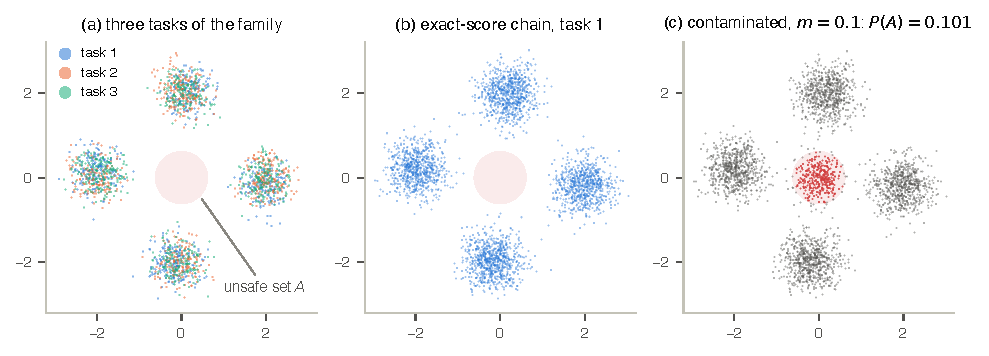
\includegraphics[width=\textwidth]{figures/fig_task_family.pdf}
\caption{Task family and unsafe set. (a) Samples of three tasks. (b) Output of the
exact-score diffusion chain of task~1, which reproduces the task. (c) Output of the chain of
the contaminated field with $m=0.1$; samples in the unsafe set $A$ are red.}
\label{fig:tasks}
\end{figure}

\subsection{The direction of the cost decides what the region excludes}

\begin{table}[!tbp]
\centering
\caption{Divergence between a contaminated field and its own clean field (median over the
pool), and probability of the unsafe set. Proposition~\ref{pr:direction} bounds the forward
divergence by $\log\frac{1}{1-m}$ for exact mixtures, and the measured values stay within a
factor of three of it; the reverse divergence exceeds it by a factor of $9$--$20$ (A) and $3$--$13$ (D). Safe fields:
$\Pv{v}(A)$ averages $\pALmean$ (A) and $\pALDmean$ (D), and the median pairwise divergence between
safe fields is $\pairKLAmed$ (A) and $\pairKLDmed$ (D) nats.}
\label{tab:kl_mass}
\small
\begin{tabular}{c c ccc ccc}
\toprule
 & & \multicolumn{3}{c}{(A) diffusion, exact scores} & \multicolumn{3}{c}{(D) linear FM, SDE}\\
\cmidrule(lr){3-5}\cmidrule(lr){6-8}
$m$ & $\log\frac1{1-m}$ & $\Pv{v}(A)$ & forward KL & reverse KL & $\Pv{v}(A)$ & forward KL & reverse KL\\
\midrule
\inputrows{tables/tab_kl_mass.tex}
\bottomrule
\end{tabular}
\end{table}

\begin{table}[!tbp]
\centering
\caption{Mean coverage of held-out safe fields (nominal $0.902$) and fraction of contaminated
fields outside the region, by unsafe mass $m$, averaged over random splits.}
\label{tab:coverage}
\small
\begin{tabular}{l c ccccc}
\toprule
cost $c(v,v_i)$ & coverage & $m=0.002$ & $0.01$ & $0.03$ & $0.1$ & $0.3$\\
\midrule
\inputrows{tables/tab_coverage.tex}
\bottomrule
\end{tabular}
\end{table}

Table~\ref{tab:coverage} and Figure~\ref{fig:exclusion} report coverage and exclusion.
Coverage is at the nominal level for every cost, as Proposition~\ref{pr:coverage} guarantees.
Exclusion depends strongly on the direction of the cost. With exact scores, the forward region
excludes only $\exclAFthree$ of the fields that carry $3\%$ unsafe mass, against $\exclAKthree$ for the
reverse-KL region, and at $m=0.01$ the rates are $\exclAFone$ against $\exclAKone$. The linear
flow-matching pilots show the same ordering ($\exclCrefthree$ against $\exclConthree$ for the ODE
sampler, $\exclDfwdthree$ against $\exclDrevthree$ for the SDE sampler at $m=0.03$), with a smaller
gap. This is consistent with the larger variation between the fitted safe fields (median pairwise
divergence $\pairKLDmed$ against $\pairKLAmed$ nats for exact scores), which widens the calibrated
budget. Figure~\ref{fig:scores} shows the mechanism on one split:
under the forward cost, the contaminated fields have scores that overlap those of the safe fields,
while under the reverse cost they are separated. Figure~\ref{fig:time} shows where in time the
reverse divergence accumulates: at the late, near-data steps, where the contaminated trajectories
are pulled into $A$ and the safe fields push them out.

\begin{figure}[!tbp]
\centering
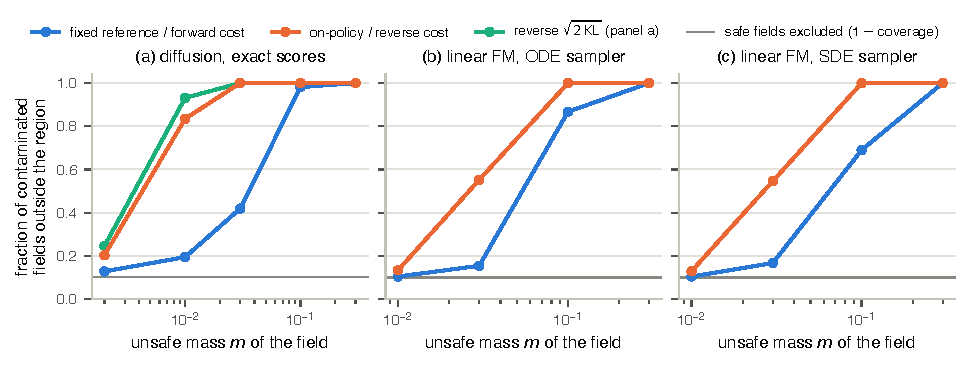
\includegraphics[width=\textwidth]{figures/fig_exclusion.pdf}
\caption{Fraction of contaminated fields outside the region as a function of their unsafe
mass. The grey line is the fraction of held-out safe fields outside the region (one minus the
coverage).}
\label{fig:exclusion}
\end{figure}

\begin{figure}[!tbp]
\centering
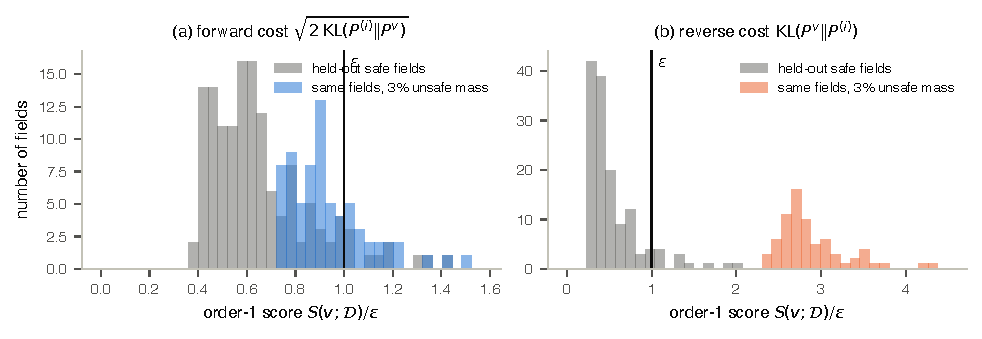
\includegraphics[width=\textwidth]{figures/fig_scores.pdf}
\caption{Order-$1$ scores, normalised by the conformal threshold, of the held-out safe fields
and of the same fields with $3\%$ unsafe mass (diffusion with exact scores, one split).}
\label{fig:scores}
\end{figure}

\begin{figure}[!tbp]
\centering
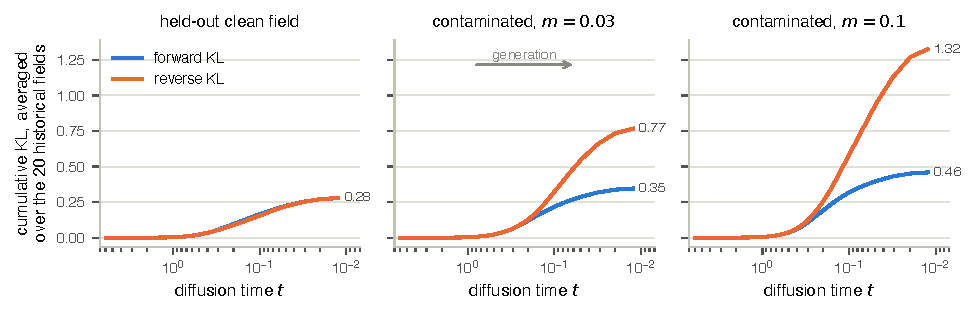
\includegraphics[width=\textwidth]{figures/fig_time_profiles.pdf}
\caption{Cumulative path divergence between a held-out field and the $20$ historical fields
(averaged over the historical fields), as generation proceeds from $t=T$ to $t_{\min}$.
Left: a clean field; middle and right: the same field with unsafe mass $m$. The final values are
the averages that enter the order-$1$ score.}
\label{fig:time}
\end{figure}

\subsection{Certificates}

\begin{table}[!tbp]
\centering
\caption{Guaranteed bound on $\Pv{v}(A)$ for every field of the region (median over splits)
and the largest actual $\Pv{v}(A)$ among the held-out and contaminated fields inside the region
(median and maximum over splits). Violations: splits where the actual value exceeds the
bound.}
\label{tab:certificates}
\small
\begin{tabular}{l c c c c}
\toprule
region and bound & bound (median) & actual (median) & actual (max) & violations\\
\midrule
\inputrows{tables/tab_certificates.tex}
\bottomrule
\end{tabular}
\end{table}

Table~\ref{tab:certificates} and Figure~\ref{fig:certificates} check the certificates of
Theorems~\ref{th:tv} and~\ref{th:rare} with the plug-in convention of Remark~\ref{rem:mc}. No
split violates a bound. The total-variation certificate is valid but loose ($\certAFmed$ with exact
scores, $\certDfwdmed$ with linear fits), because total variation cannot use the rarity of $A$. The
reverse-KL certificate of Theorem~\ref{th:rare} is $\certAKmed$ with exact scores, within a factor of
three of the worst field actually inside the region ($\insideAKmed$), and $\certDrevmed$ with linear
fits (worst field $\insideDrevmed$). The difference between the two pilots is the floor of
Remark~\ref{rem:floor}: the linear fits are more spread out in divergence, so the calibrated budget
$(M+1)\varepsilon$ is larger.

\begin{figure}[!tbp]
\centering
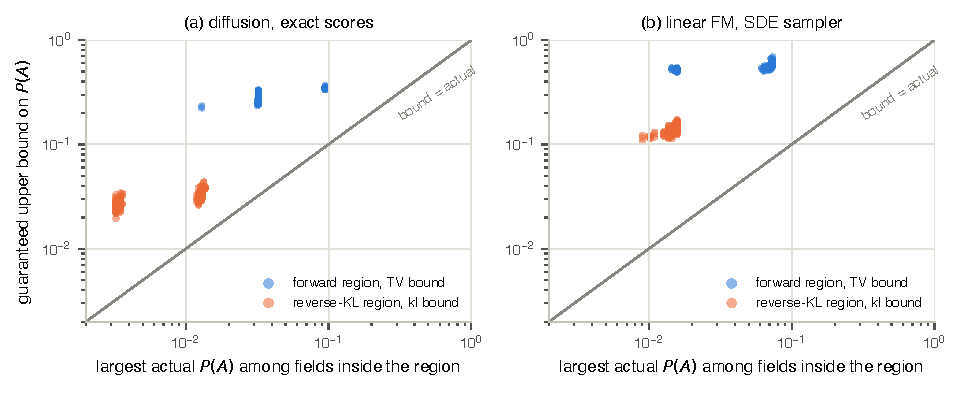
\includegraphics[width=\textwidth]{figures/fig_certificates.pdf}
\caption{Each point is one random split: largest actual $\Pv{v}(A)$ among the fields inside the
region against the guaranteed bound. Points above the diagonal are valid certificates.}
\label{fig:certificates}
\end{figure}

\subsection{Few-shot fine-tuning with linear flow matching}

\begin{table}[!tbp]
\centering
\caption{Few-shot fine-tuning on $\ntasks$ held-out tasks ($12$ clean samples, and $12$ clean plus
$3$ unsafe samples). MMD$^2$ is multiplied by $10^3$. The last two columns give the fraction of
fitted fields inside the fixed-Gram region and inside the on-policy region (contaminated case).}
\label{tab:fewshot}
\small
\begin{tabular}{l cc cc cc}
\toprule
 & \multicolumn{2}{c}{clean data} & \multicolumn{2}{c}{contaminated data} & \multicolumn{2}{c}{inside region}\\
\cmidrule(lr){2-3}\cmidrule(lr){4-5}\cmidrule(lr){6-7}
estimator & MMD$^2$ & $\Pv{v}(A)$ & MMD$^2$ & $\Pv{v}(A)$ & fixed $G$ & on-policy\\
\midrule
\inputrows{tables/tab_fewshot.tex}
\bottomrule
\end{tabular}
\end{table}

Table~\ref{tab:fewshot} and Figure~\ref{fig:fewshot} summarise the few-shot study, and
Figures~\ref{fig:samples}--\ref{fig:trajectories} show one task (test task $\exampletask$). Three
observations follow.

\emph{The constraint helps against least squares.} The conformal SOCP beats the best
least-squares fit on $\winCrefclean/\ntasks$ tasks with clean data and $\winCrefcont/\ntasks$ with
contaminated data, with geometric-mean MMD$^2$ ratios $\geoCrefclean$ and $\geoCrefcont$; the
on-policy variant gives $\geoConclean$ and $\geoConcont$. Each SOCP takes $\socptime$\,s.

\emph{The constraint limits the unsafe mass, and the on-policy cost limits it more.} With $20\%$
contaminated samples, least squares puts $\pAUcont$ of its mass in $A$, the fixed-Gram constraint
$\pACrefcont$ and the on-policy constraint $\pAConcont$ (historical safe fits: $\pALCmean$). The
fixed-Gram solutions are inside the fixed-Gram region but never inside the on-policy region,
i.e.\ the on-policy region detects their contamination. Algorithm~\ref{alg:scp} ended slightly
infeasible in a fraction $\backofffrac$ of the runs, and the back-off then moved the solution by at
most $\backoffmax$ of the way to the centre.

\emph{In this concentrated family, strong shrinkage towards the centre is better still.} The centre
alone, which uses no data, is within a factor of two of the oracle in MMD$^2$, and shrinkage with
$\gamma=10$ (tuned on the test tasks, an optimistic baseline) beats the conformal estimators in
accuracy and in unsafe mass ($\pASten$). With $12$ samples the least-squares objective pulls the
constrained solution onto the boundary of the region, which is calibrated to contain $90\%$ of the
legitimate tasks and is therefore wide compared with the information in $12$ samples. The neural
network study of the manuscript (gauge versus projected gradient at $n\leq5$) shows the same
behaviour. The region is a safety and validity device, not an estimator by itself; combining it with
shrinkage inside the region, $\min_{\bth}\hat L(\bth)+\gamma S(\bth;\cD)$ subject to
$S(\bth;\cD)\leq\varepsilon$, keeps the certificate and should recover the accuracy (not tested here).

\begin{figure}[!tbp]
\centering
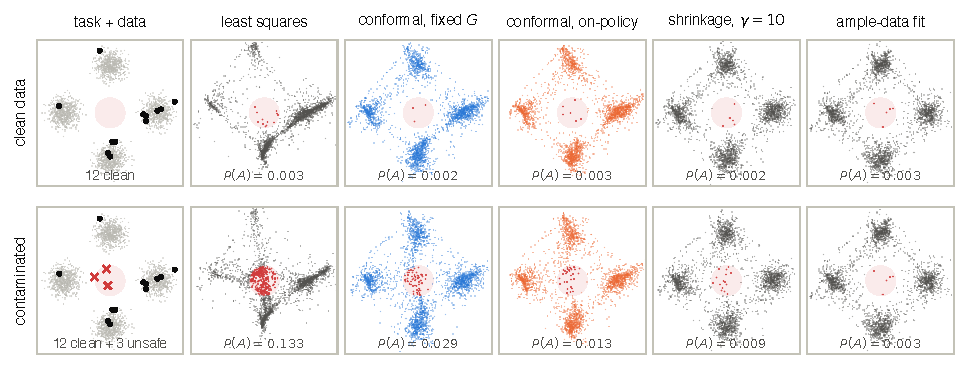
\includegraphics[width=\textwidth]{figures/fig_samples.pdf}
\caption{Generated samples for test task~$\exampletask$. First column: the clean task (grey) and the
few-shot data (black, unsafe samples as red crosses). Other columns: ODE samples of each fitted
field; samples in $A$ are red. Top: clean data; bottom: contaminated data.}
\label{fig:samples}
\end{figure}

\begin{figure}[!tbp]
\centering
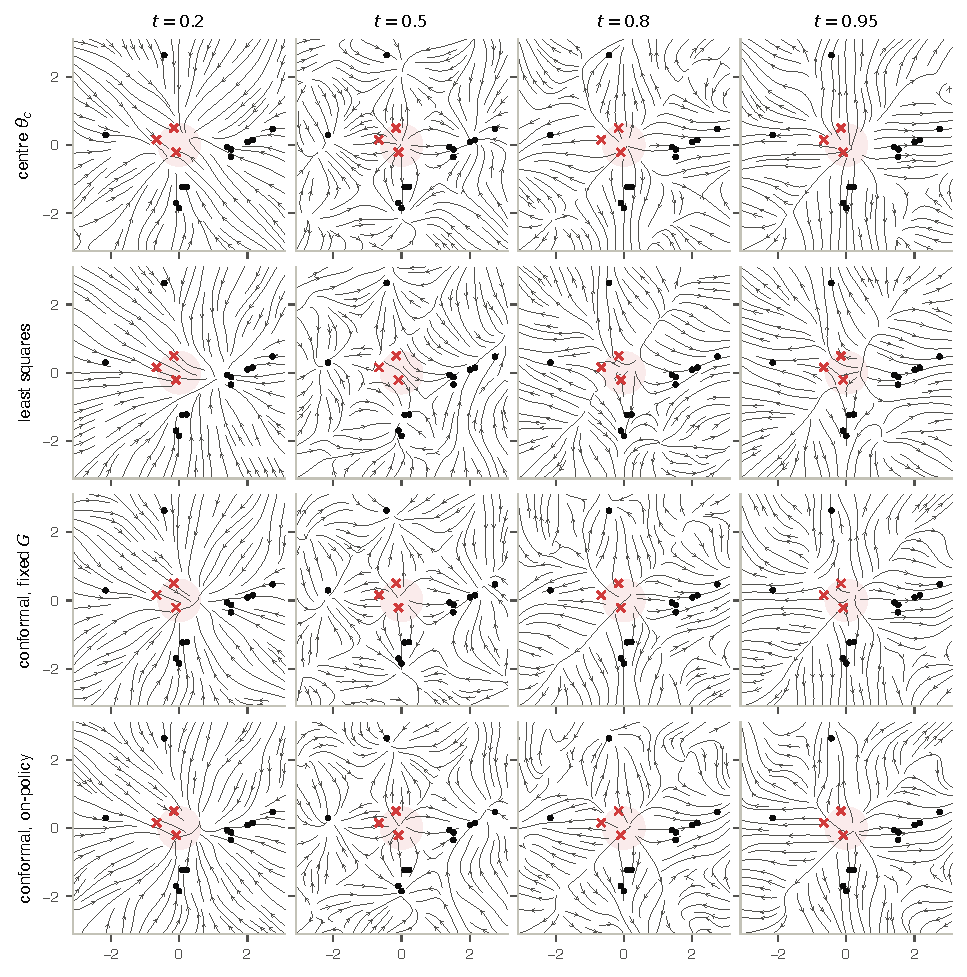
\includegraphics[width=\textwidth]{figures/fig_fields.pdf}
\caption{Streamlines of the time-dependent velocity fields $v_{\bth}(\cdot,t)$ fitted on the
contaminated data of test task~$\exampletask$, at four times. Early on ($t=0.2$) every field
contracts the noise towards the origin; the fields differ at late times. Least squares develops
sinks at the unsafe samples inside $A$ (red disk); the constrained fields route the flow to the
ring.}
\label{fig:fields}
\end{figure}

\begin{figure}[!tbp]
\centering
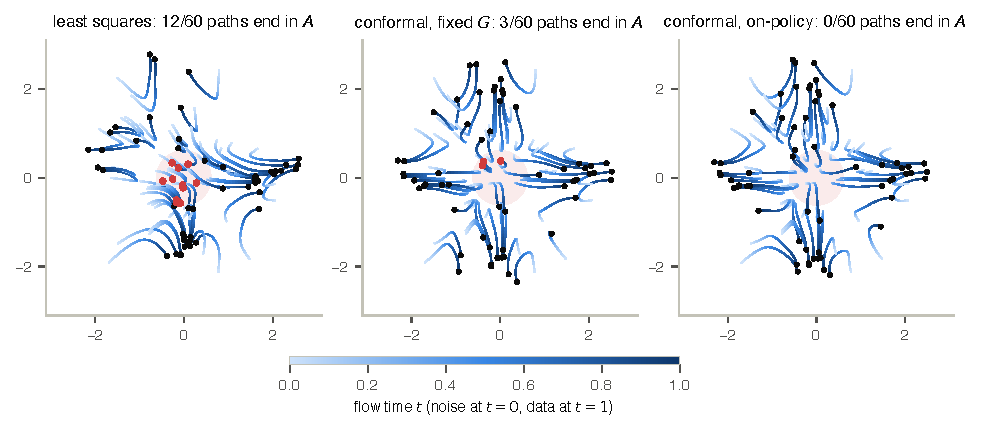
\includegraphics[width=\textwidth]{figures/fig_trajectories.pdf}
\caption{Sixty ODE trajectories of the fields of Figure~\ref{fig:fields}, coloured by time;
end points in $A$ are red.}
\label{fig:trajectories}
\end{figure}

\begin{figure}[!tbp]
\centering
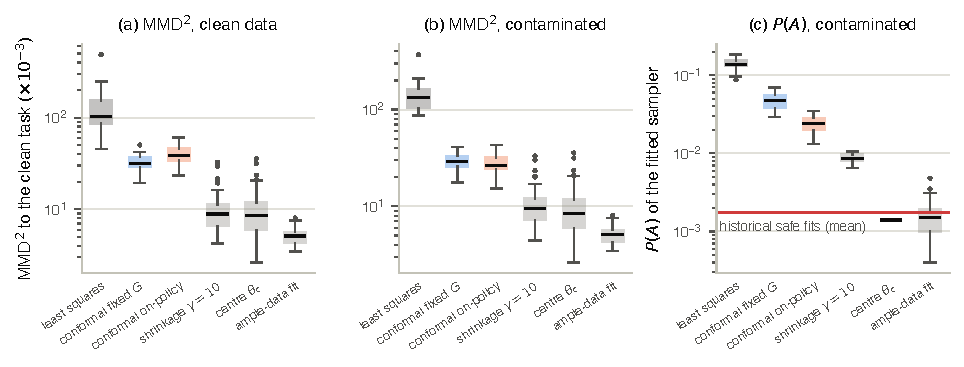
\includegraphics[width=\textwidth]{figures/fig_fewshot.pdf}
\caption{Few-shot fine-tuning over $\ntasks$ held-out tasks: MMD$^2$ to the clean task with clean
data (a) and with contaminated data (b), and probability of the unsafe set with contaminated data
(c). The red line is the mean over the historical safe fits.}
\label{fig:fewshot}
\end{figure}

% =====================================================================================
\section{Prompt-conditioned flow matching: safe prompts induce safe fields}\label{sec:prompts}
% =====================================================================================

This section specialises the construction to the setting that motivates it: a trained
text-to-image (or text-to-action) flow-matching model whose velocity field is shaped by the
embedding of a prompt. The model is fixed and only the prompt varies, so a collection of safe
prompts yields a collection of safe vector fields, and the order-$1$ region is built on these
fields.

\paragraph{Setting.}
Let $v(\bx,t;\be)$ be a trained velocity field conditioned on a prompt embedding
$\be\in\mathcal{E}\subseteq\RR^p$ (for a tokenised prompt, the flattened output of a fixed text
encoder). Each prompt defines a field $v_{\be}\coloneqq v(\cdot,\cdot;\be)$. The safe training
prompts $\be_1,\dots,\be_M$ define the safe fields $v_{\be_1},\dots,v_{\be_M}$, and the calibration
prompts $\be_{M+1},\dots,\be_{M+K}$ define the calibration fields; all are drawn from a distribution
of approved prompts. A new prompt $\be$ may be unsafe, or adversarial. Let
$\mu_0\coloneqq\mathcal{N}(0,I_n)$ and let $T_{\be}:\RR^n\to\RR^n$ map the initial noise $\bx_0$ to the
output of the deterministic sampler (the exact flow map, or the $J$-step Euler map). A fixed
measurable map $\chi:\RR^n\to\RR^q$ (the identity, a decoder, an image encoder, or the features of
a safety classifier) chooses the space in which outputs are compared. A cost on fields is pulled
back to prompts, $c(\be,\be')\coloneqq c(v_{\be},v_{\be'})$, and the order-$1$ score of a prompt is
$S^w_c(\be;\cD)=\frac{1}{M+1}\sum_iw_i\,c(\be,\be_i)$ as in Definition~\ref{def:score}.

\subsection{Straight flows: when time collapses}\label{subsec:straight}

\begin{definition}[Straight flow, one-step map, straightness defect]\label{def:straight}
The field $v_{\be}$ is \emph{straight} if every trajectory of $\dot X_t=v_{\be}(X_t,t)$ is a segment
traversed at constant speed: $X_t=X_0+t\,(X_1-X_0)$ for all $t\in[0,1]$. The \emph{one-step map}
is $\tilde T_{\be}(\bx_0)\coloneqq\bx_0+v_{\be}(\bx_0,0)$ and the \emph{straightness defect} is
$\zeta_{\be}\coloneqq\|T_{\be}-\tilde T_{\be}\|_{L^2(\mu_0)}$, where
$\|F\|_{L^2(\mu_0)}\coloneqq(\E_{\bx_0\sim\mu_0}\|F(\bx_0)\|^2)^{1/2}$.
\end{definition}

\begin{lemma}[Straight flows]\label{lem:straight}
Let $v_{\be}$ and $v_{\be'}$ be straight, let $\bx_0\in\RR^n$, and let $X^{\be}_t$ and $X^{\be'}_t$ be
their trajectories from $\bx_0$. Then:
(i) $v_{\be}(X^{\be}_t,t)=v_{\be}(\bx_0,0)$ for all $t$: along each trajectory the velocity is
constant, in direction and in magnitude;
(ii) $T_{\be}=\tilde T_{\be}$, i.e.\ $\zeta_{\be}=0$, and $X^{\be}_t=\bx_0+t\,v_{\be}(\bx_0,0)$;
(iii) $\sup_{t\in[0,1]}\|X^{\be}_t-X^{\be'}_t\|=\|v_{\be}(\bx_0,0)-v_{\be'}(\bx_0,0)\|$ and
$\int_0^1\|v_{\be}(X^{\be}_t,t)-v_{\be'}(X^{\be'}_t,t)\|^2\,dt=\|v_{\be}(\bx_0,0)-v_{\be'}(\bx_0,0)\|^2$;
(iv) at a fixed point $\bx$, $t\mapsto v_{\be}(\bx,t)$ need not be constant, in direction or in
magnitude. For instance, the field with $v(\bx,0)=A\bx$ and
$A=\big(\begin{smallmatrix}0&-1\\1&0\end{smallmatrix}\big)$ is straight, $v(\bx,t)=A(I+tA)^{-1}\bx$, and at
$\bx=(1,0)$ its direction rotates from $90^\circ$ at $t=0$ to $45^\circ$ at $t=1$.
\end{lemma}
\textit{Proof:}
(i) By Definition~\ref{def:straight}, $X^{\be}_t=\bx_0+t(X^{\be}_1-\bx_0)$, so
$\dot X^{\be}_t=X^{\be}_1-\bx_0$ does not depend on $t$. Since $\dot X^{\be}_t=v_{\be}(X^{\be}_t,t)$, the
velocity along the trajectory equals its value at $t=0$, which is $v_{\be}(\bx_0,0)$.
(ii) By (i), $X^{\be}_1-\bx_0=v_{\be}(\bx_0,0)$, i.e.\ $T_{\be}(\bx_0)=\tilde T_{\be}(\bx_0)$; the trajectory then
follows from Definition~\ref{def:straight}.
(iii) By (ii), $X^{\be}_t-X^{\be'}_t=t\,(v_{\be}(\bx_0,0)-v_{\be'}(\bx_0,0))$, whose norm is largest at $t=1$.
By (i), the integrand of the second identity does not depend on $t$ and equals
$\|v_{\be}(\bx_0,0)-v_{\be'}(\bx_0,0)\|^2$.
(iv) The trajectories of the example are $X_t=(I+tA)\bx_0$, segments traversed at the constant
speed $A\bx_0$, so the field is straight. The matrix $I+tA$ is invertible (its eigenvalues are
$1\pm it$), so the point $\bx$ is reached at time $t$ from $\bx_0=(I+tA)^{-1}\bx$, and
$v(\bx,t)=A\bx_0=A(I+tA)^{-1}\bx$. With
$(I+tA)^{-1}=\frac{1}{1+t^2}\big(\begin{smallmatrix}1&t\\-t&1\end{smallmatrix}\big)$ one gets
$v((1,0),t)=\frac{1}{1+t^2}(t,1)$, whose angle with the first axis is $\arctan(1/t)$.
\hfill $\square$

Lemma~\ref{lem:straight} makes precise the intuition that in a straight (``linear'') flow the
field does not change angle through time: this holds \emph{along trajectories}, not at a fixed
point. Its practical content is (ii)--(iii). For a straight flow the whole time-dependent field is
summarised by its slice at $t=0$, the sampler is a single step, and every time-integrated
comparison of two fields along their own trajectories reduces to a comparison of these slices.

\begin{remark}[The linear interpolant does not make the learned flow straight]\label{rem:not_straight}
Training with the linear interpolant on independent noise/data pairs makes the
\emph{conditional} paths straight, not the learned marginal flow. Already for Gaussian data
$\mathcal{N}(0,\Sigma)$, with $C_t\coloneqq(1-t)^2I+t^2\Sigma$, the marginal velocity is
$v^\star(\bx,t)=(t\Sigma-(1-t)I)\,C_t^{-1}\bx$ (Gaussian conditioning, since
$\mathrm{Cov}(\bx_1-\bx_0,\bx_t)=t\Sigma-(1-t)I$), and its flow is $X_t=C_t^{1/2}X_0$: indeed
$\frac{d}{dt}C_t^{1/2}=\frac12C_t^{-1/2}\dot C_t=(t\Sigma-(1-t)I)\,C_t^{-1/2}$, because all the
matrices involved commute. In an eigenbasis of $\Sigma$ the $j$-th coordinate is scaled by
$\sqrt{(1-t)^2+t^2\lambda_j}$, which is not affine in $t$, so the trajectories are not segments;
when the eigenvalues differ, the direction of $X_t$ changes as well. Reflow \citep{liu2023flow}
straightens the coupling; one-step text-to-image generators are obtained by reflow and
distillation \citep{liu2024instaflow}; text-to-image models trained with the rectified-flow
objective \citep{esser2024scaling} are not reflowed, so their flows need not be straight. The defect
$\zeta_{\be}$ measures the deviation, and it enters the bounds below.
\end{remark}

\subsection{Map metrics and their certificate}\label{subsec:map_metrics}

\begin{definition}[Map metrics]\label{def:map_metrics}
For prompts $\be,\be'$ let
\[
  d_T(\be,\be')\coloneqq\|T_{\be}-T_{\be'}\|_{L^2(\mu_0)},\qquad
  d_0(\be,\be')\coloneqq\|\tilde T_{\be}-\tilde T_{\be'}\|_{L^2(\mu_0)}=\|v_{\be}(\cdot,0)-v_{\be'}(\cdot,0)\|_{L^2(\mu_0)},
\]
\[
  d_\chi(\be,\be')\coloneqq\|\chi\circ T_{\be}-\chi\circ T_{\be'}\|_{L^2(\mu_0)} .
\]
\end{definition}

\begin{lemma}[Map metrics are pseudometrics]\label{lem:map_metrics}
$d_T$, $d_0$ and $d_\chi$ are pseudometrics on prompts (equivalently, on fields), and
$|d_T(\be,\be')-d_0(\be,\be')|\leq\zeta_{\be}+\zeta_{\be'}$. In particular $d_T=d_0$ on straight fields.
\end{lemma}
\textit{Proof:}
Each is the $L^2(\mu_0)$ distance between two functions of $\bx_0$; it is therefore symmetric,
zero on the diagonal, and satisfies the triangle inequality of the $L^2(\mu_0)$ norm. For the
bound, the triangle inequality in $L^2(\mu_0)$ gives
$\|T_{\be}-T_{\be'}\|\leq\|T_{\be}-\tilde T_{\be}\|+\|\tilde T_{\be}-\tilde T_{\be'}\|+\|\tilde T_{\be'}-T_{\be'}\|$, i.e.\
$d_T\leq\zeta_{\be}+d_0+\zeta_{\be'}$, and symmetrically $d_0\leq\zeta_{\be}+d_T+\zeta_{\be'}$. By
Lemma~\ref{lem:straight}(ii), $\zeta=0$ on straight fields. \hfill $\square$

By Lemma~\ref{lem:closed_form}, the order-$1$ score with any of these costs is exactly the order-$1$
Wasserstein distance between consecutive empirical distributions whose samples are the safe
fields, with the metric defined on the space of fields. In practice the outputs
$\chi(T_{\be_i}(\bx_0^{(l)}))$ of the safe prompts on a fixed set of probe noises
$\bx_0^{(1)},\dots,\bx_0^{(L)}$ are computed once and stored. Scoring a new prompt then costs one run of
the sampler on the probe noises (one network evaluation per probe for $d_0$), plus the encoder
$\chi$. The memory is $M\times L\times q$ numbers, which favours a low-dimensional $\chi$.

\begin{theorem}[Output certificate for map metrics]\label{th:map_cert}
Let $d=d_\chi$ (with $\chi=\mathrm{id}$, $d=d_T$), let $w$ be a probability vector and
$\varepsilon\geq0$, and assume $S^w_d(\be;\cD)\leq\varepsilon$. Let $\bx_0\sim\mu_0$ and $I\sim w$ be independent,
$Y\coloneqq\chi(T_{\be}(\bx_0))$ and $Y'\coloneqq\chi(T_{\be_I}(\bx_0))$. Then:
(i) $Y$ has the law of the (encoded) outputs of the prompt $\be$, $Y'$ has the $w$-mixture of the laws
of the outputs of the safe prompts, and $\E\|Y-Y'\|\leq(M+1)\varepsilon$; hence
$W_1(\mathrm{law}(Y),\mathrm{law}(Y'))\leq(M+1)\varepsilon$;
(ii) for every Borel set $B\subseteq\RR^q$ and every $r>0$, with $B^{+r}\coloneqq\{\by:\dist(\by,B)<r\}$,
\[
  \mathbbm{P}\big(\chi(T_{\be}(\bx_0))\in B\big)\;\leq\;\sum_iw_i\,\mathbbm{P}\big(\chi(T_{\be_i}(\bx_0))\in B^{+r}\big)+\frac{(M+1)\varepsilon}{r};
\]
(iii) if the region is defined with $d_0$ instead (i.e.\ $S^w_{d_0}(\be;\cD)\leq\varepsilon$) and
$\chi=\mathrm{id}$, then (i)--(ii) hold for the outputs of the full sampler with $(M+1)\varepsilon$ replaced
by $(M+1)\varepsilon+\zeta_{\be}+\sum_iw_i\zeta_{\be_i}$.
\end{theorem}
\textit{Proof:}
(i) The marginal statements follow from the independence of $\bx_0$ and $I$. Conditioning on $I$ and
using $\E\|Z\|\leq(\E\|Z\|^2)^{1/2}$,
$\E\|Y-Y'\|=\sum_iw_i\,\E\|\chi(T_{\be}(\bx_0))-\chi(T_{\be_i}(\bx_0))\|\leq\sum_iw_i\,d_\chi(\be,\be_i)$, which
is at most $(M+1)\varepsilon$ by \eqref{eq:budget}. Since $(Y,Y')$ is a coupling of the two laws, $W_1$ is
at most $\E\|Y-Y'\|$.
(ii) As in Step~4 of Proposition~\ref{pr:ode}: if $Y\in B$ and $\|Y-Y'\|<r$, then $Y'\in B^{+r}$, so
$\mathbbm{P}(Y\in B)\leq\mathbbm{P}(Y'\in B^{+r})+\mathbbm{P}(\|Y-Y'\|\geq r)$; Markov's inequality and
(i) bound the last term by $(M+1)\varepsilon/r$.
(iii) By Lemma~\ref{lem:map_metrics}, $d_T(\be,\be_i)\leq d_0(\be,\be_i)+\zeta_{\be}+\zeta_{\be_i}$; multiplying by
$w_i$ and summing, $\sum_iw_id_T(\be,\be_i)\leq(M+1)\varepsilon+\zeta_{\be}+\sum_iw_i\zeta_{\be_i}$. Repeat (i)--(ii)
with this bound. \hfill $\square$

Theorem~\ref{th:map_cert} is Proposition~\ref{pr:ode} with the Gr\"onwall factor replaced by $1$:
comparing outputs under shared noise, instead of fields along trajectories, removes the propagation
of errors that made Proposition~\ref{pr:ode} vacuous. The certificate holds deterministically for every
prompt whose score is at most $\varepsilon$, safe or not, and for every set $B$ at once, so the method
never needs to know $B$. Its strength depends on two things: the budget $(M+1)\varepsilon$, which the floor
of Remark~\ref{rem:floor} ties to the spread of the safe prompts, and the space in which outputs are
compared, which $\chi$ chooses. A pixel or latent distance is not semantic; a fixed image encoder
makes the certificate semantic in its feature space.

\begin{proposition}[Sensitivity of map metrics to rare unsafe outputs]\label{pr:sqrt_m}
Let $\Delta_{\mathrm{s}}>0$ and let $N\subseteq\RR^n$ be a set of noises with $\mu_0(N)=m$ such that
$\|\chi(T_{\be}(\bx))-\chi(T_{\be_i}(\bx))\|\geq\Delta_{\mathrm{s}}$ for all $\bx\in N$ and all
$i\in\llbracket M\rrbracket$. Then $d_\chi(\be,\be_i)\geq\sqrt m\,\Delta_{\mathrm{s}}$ for every $i$, hence
$S_{d_\chi}(\be;\cD)\geq\sqrt m\,\Delta_{\mathrm{s}}/(M+1)$, and $\be$ lies outside the region whenever
$\sqrt m\,\Delta_{\mathrm{s}}>(M+1)\varepsilon$.
\end{proposition}
\textit{Proof:}
$d_\chi(\be,\be_i)^2=\int\|\chi T_{\be}-\chi T_{\be_i}\|^2d\mu_0\geq\int_N\|\chi T_{\be}-\chi T_{\be_i}\|^2d\mu_0\geq m\Delta_{\mathrm{s}}^2$.
Averaging over $i$ with weights $1/M$ and dividing by $M+1$ gives the bound on the score. \hfill $\square$

A prompt that sends a fraction $m$ of the noise to outputs at distance $\Delta_{\mathrm{s}}$ from the safe
outputs therefore costs at least $\sqrt m\,\Delta_{\mathrm{s}}$ under a map metric, compared with at most
$\log\frac{1}{1-m}\approx m$ under a forward divergence (Proposition~\ref{pr:direction}). Map metrics
detect rare unsafe outputs when these are far from the safe outputs in the space chosen by $\chi$.
They do not use the rarity of the unsafe region; only the reverse divergence of
Theorem~\ref{th:rare} does.

\subsection{Forcing a prompt into the safe set}\label{subsec:forcing}

A prompt whose score exceeds $\varepsilon$ can be refused, or its field can be moved into the region.
Two mechanisms have closed forms.

\begin{proposition}[One-step blending]\label{pr:blend}
Let $\be_c$ be a prompt with $S_{d_0}(\be_c;\cD)<\varepsilon<S_{d_0}(\be;\cD)$ (for instance the safe
training prompt nearest to $\be$ among those whose in-sample score is below $\varepsilon$). For
$\lambda\in[0,1]$ let $\tilde T_\lambda\coloneqq(1-\lambda)\tilde T_{\be}+\lambda\tilde T_{\be_c}$, that is,
$\tilde T_\lambda(\bx_0)=\bx_0+(1-\lambda)v(\bx_0,0;\be)+\lambda v(\bx_0,0;\be_c)$, and
$S(\lambda)\coloneqq\frac{1}{M(M+1)}\sum_i\|\tilde T_\lambda-\tilde T_{\be_i}\|_{L^2(\mu_0)}$. Then $S$ is convex
on $[0,1]$, and
$\lambda^\star\coloneqq\frac{S_{d_0}(\be;\cD)-\varepsilon}{S_{d_0}(\be;\cD)-S_{d_0}(\be_c;\cD)}\in(0,1)$ satisfies
$S(\lambda^\star)\leq\varepsilon$. Consequently the one-step outputs $\tilde T_{\lambda^\star}(\bx_0)$ satisfy
Theorem~\ref{th:map_cert}(i)--(ii) with respect to the one-step outputs of the safe prompts.
\end{proposition}
\textit{Proof:}
$\tilde T_\lambda-\tilde T_{\be_i}=(1-\lambda)(\tilde T_{\be}-\tilde T_{\be_i})+\lambda(\tilde T_{\be_c}-\tilde T_{\be_i})$ is
affine in $\lambda$, so each norm, and hence their sum, is convex in $\lambda$. Since $S(0)=S_{d_0}(\be;\cD)$
and $S(1)=S_{d_0}(\be_c;\cD)$, Proposition~\ref{pr:backoff} (convex case) gives $S(\lambda^\star)\leq\varepsilon$.
The map $\tilde T_{\lambda^\star}$ plays the role of $T_{\be}$ in Theorem~\ref{th:map_cert} with $\chi=\mathrm{id}$,
and the proof of the theorem applies verbatim. \hfill $\square$

The blend costs two network evaluations, as classifier-free guidance does
\citep{ho2022classifier}, and for a straight model it is the whole sampler. With a multi-step sampler,
blending the velocities at every step does not blend the maps, because the flow is nonlinear.
The bisection of Proposition~\ref{pr:backoff}, run on $d_T$ with the blended sampler re-simulated on
the probe noises, nevertheless returns a field inside the region, since its invariant needs no
convexity. The choice of $\be_c$ trades fidelity against cost. The nearest feasible safe prompt keeps
as much of the request as the region allows. The geometric median of the safe maps, which is a
convex combination $\sum_j\alpha_j\tilde T_{\be_j}$ of them because $L^2(\mu_0)$ is a Hilbert space, requires
$M$ network evaluations per step.

\begin{proposition}[Prompt projection for a model affine in the prompt]\label{pr:prompt_proj}
Assume $v(\bx,0;\be)=\mathbf{a}(\bx)+J(\bx)\be$ for all $\be$, with $J(\bx)\in\RR^{n\times p}$ and
$\E_{\mu_0}\|J\|_F^2<\infty$; let $G_J\coloneqq\E_{\mu_0}[J^\top J]$ and assume $G_J\succ0$. Then:
(i) $d_0(\be,\be')=\|\be-\be'\|_{G_J}$, the pull-back of the field metric to prompt embeddings;
(ii) if $S_{d_0}(\be_c;\cD)<\varepsilon$ for some $\be_c$ and $R\coloneqq M(M+1)\varepsilon$, the projection
\[
  \be^\star\coloneqq\argmin_{\be\in\RR^p}\ \|\be-\be_{\mathrm{new}}\|_{G_J}^2\quad\text{s.t.}\quad\sum_{i=1}^M\|\be-\be_i\|_{G_J}\leq R
\]
exists, is unique, solves a second-order cone program, and its field lies in the region;
(iii) $\be^\star$ belongs to the convex hull of $\{\be_{\mathrm{new}},\be_1,\dots,\be_M\}$, so it can be computed over
the simplex of $\RR^{M+1}$ from the Gram matrix $K_{ab}\coloneqq\be_a^\top G_J\be_b$, $a,b\in\{0,\dots,M\}$,
$\be_0\coloneqq\be_{\mathrm{new}}$, whatever the embedding dimension $p$.
\end{proposition}
\textit{Proof:}
(i) $v(\cdot,0;\be)-v(\cdot,0;\be')=J(\be-\be')$; take the squared norm and the expectation, as in
Proposition~\ref{pr:mahalanobis}(a).
(ii) The feasible set is closed, convex and non-empty (it contains $\be_c$), and the objective is
strictly convex and coercive because $G_J\succ0$, so the minimiser exists and is unique; the
second-order cone reformulation is that of Proposition~\ref{pr:socp}. By (i), the constraint reads
$S_{d_0}(\be^\star;\cD)\leq\varepsilon$.
(iii) If the constraint is inactive, $\be^\star=\be_{\mathrm{new}}$; if $\be^\star=\be_j$ for some $j$, the claim is
immediate. Otherwise the constraint function is differentiable at $\be^\star$, Slater's condition holds
because $\be_c$ is strictly feasible, and the Karush--Kuhn--Tucker conditions give a multiplier
$\nu\geq0$ with $2G_J(\be^\star-\be_{\mathrm{new}})+\nu\sum_iG_J(\be^\star-\be_i)/r_i=0$, where
$r_i\coloneqq\|\be^\star-\be_i\|_{G_J}>0$. Multiplying by $G_J^{-1}$ and solving,
$\be^\star=\big(2\be_{\mathrm{new}}+\nu\sum_i\be_i/r_i\big)/\big(2+\nu\sum_i1/r_i\big)$, a convex combination. Writing
$\be=\sum_a\alpha_a\be_a$, every norm in the problem is
$\|\be-\be_b\|_{G_J}^2=(\boldsymbol{\alpha}-\mathbf{1}_b)^\top K(\boldsymbol{\alpha}-\mathbf{1}_b)$, with $\mathbf{1}_b$ the
$b$-th unit vector. \hfill $\square$

For a model that is not affine in the prompt, $J$ is the Jacobian of $v(\bx,0;\cdot)$ at
$\be_{\mathrm{new}}$, the projection is exact to first order only, and the score of the projected prompt must
be checked on the true model, with the back-off of Proposition~\ref{pr:backoff} if it exceeds $\varepsilon$.
The entries of $K$ require only Jacobian--vector products $J(\bx)\be_a$ on the probe noises, $M+1$ per
probe.

\subsection{Local safe sets for diverse prompts}\label{subsec:local}

When the safe prompts are diverse, the floor of Remark~\ref{rem:floor} makes the uniform region wide:
its budget is at least half the mean distance between, say, the fields of a prompt about a cat and of a
prompt about a car, and forcing then pulls towards an ``average'' safe output. Two localisations keep
the guarantees.

\emph{Prompt-adaptive weights.} Let the weights depend on the new prompt, e.g.\
$w_i(\be)\propto\exp(-\|\be-\be_i\|^2/(2h^2))$, or uniform on the $k$ safe prompts nearest to $\be$ in embedding
space, as in the task-adaptive score $g_{d,1}$ of the manuscript. The map $\be\mapsto S^{w(\be)}_d(\be;\cD)$ is
still a fixed function of the prompt once the training prompts are fixed. Proposition~\ref{pr:coverage}
therefore applies when every calibration prompt is scored with its own weights, and
Theorem~\ref{th:map_cert} holds with the $w(\be)$-mixture, i.e.\ relative to the safe prompts most similar to
the request.

\emph{Order-$\infty$.} The manuscript proves (\texttt{thm:regions} of its region-equivalence section,
valid for any symmetric $d$) that the order-$\infty$ region without cuts is the union of the closed
$d$-balls of radius $\varepsilon_\infty$ around the safe fields whenever $\varepsilon_\infty$ is at least the bottleneck of
the minimum spanning tree of the safe fields, i.e.\ whenever their threshold graph at level $\varepsilon_\infty$ is
connected. If $d_\chi(\be,\be_j)\leq\varepsilon_\infty$ for some $j$, the proof of Theorem~\ref{th:map_cert} with
$w$ the Dirac mass at $j$ gives
$\mathbbm{P}(\chi(T_{\be}(\bx_0))\in B)\leq\max_j\mathbbm{P}(\chi(T_{\be_j}(\bx_0))\in B^{+r})+\varepsilon_\infty/r$: the
request is certified relative to \emph{one} safe prompt, not to the average of all of them.

% =====================================================================================
\section{A catalogue of design choices}\label{sec:catalogue}
% =====================================================================================

The construction has four independent components: the cost between fields, the shape of the region,
the enforcement mechanism and the calibration procedure. This section lists the options that the
analysis supports, with the guarantee each one carries.

\subsection{Costs between fields}\label{subsec:costs}

All certificates of this note follow from one principle.

\begin{lemma}[Convexity principle]\label{lem:convexity}
Let $\mathfrak{D}$ be a $[0,+\infty]$-valued function of pairs of probability measures that is convex in its
second argument: $\mathfrak{D}(P,\sum_iw_iQ_i)\leq\sum_iw_i\mathfrak{D}(P,Q_i)$. If
$c(v,v_i)\coloneqq\mathfrak{D}(\Pv{v},P^{(i)})$ and $S^w_c(v;\cD)\leq\varepsilon$, then
$\mathfrak{D}(\Pv{v},\Pbar_w)\leq(M+1)\varepsilon$.
\end{lemma}
\textit{Proof:}
$\mathfrak{D}(\Pv{v},\Pbar_w)\leq\sum_iw_i\mathfrak{D}(\Pv{v},P^{(i)})=(M+1)S^w_c(v;\cD)\leq(M+1)\varepsilon$, by convexity
and \eqref{eq:budget}. \hfill $\square$

The hypothesis holds for: the total variation and the reverse divergence $\KL(P\|\cdot)$ (Step~1 of
Theorems~\ref{th:tv} and~\ref{th:rare}); the forward divergence $\mathfrak{D}(P,Q)\coloneqq\KL(Q\|P)$ (joint
convexity of the relative entropy); $W_1$ (a mixture of couplings of the pairs $(P,Q_i)$ is a coupling
of $(P,\sum_iw_iQ_i)$); the maximum mean discrepancy
$\mathrm{MMD}_k(P,Q)=\|\mu_P-\mu_Q\|_{\mathcal{H}_k}$, a norm of a difference of mean embeddings
\citep{gretton2012kernel}; and $|\E_Pg-\E_Qg|$ for a fixed function $g$. What the certificate means
depends on $\mathfrak{D}$:
\begin{itemize}
\item a forward divergence certifies that the candidate \emph{covers} the safe behaviour
($\KL(\Pbar_w\|\Pv{v})$ small);
\item a reverse divergence certifies that it \emph{avoids} what the safe samplers avoid;
\item $W_1$ certifies that its outputs are close to theirs.
\end{itemize}
Table~\ref{tab:costs} lists the costs.

\begin{table}[!tbp]
\centering
\caption{Costs between fields. ``Metric'': the cost is a pseudometric, so Lemma~\ref{lem:closed_form} gives
the order-$1$ Wasserstein interpretation. ``Convex'': in the field (or in the parameters of a linear
model). Last column: what the cost charges for a fraction $m$ of outputs in a region of safe
probability $q$ (with $p\geq m$ the candidate's probability of that region), at distance $\Delta_{\mathrm{s}}$
from the safe outputs.}
\label{tab:costs}
\footnotesize
\begin{tabularx}{\textwidth}{>{\raggedright\arraybackslash}p{2.3cm} >{\raggedright\arraybackslash}X c c >{\raggedright\arraybackslash}p{2.7cm} >{\raggedright\arraybackslash}p{2.3cm}}
\toprule
cost & definition & metric & convex & certificate & unsafe mass $m$\\
\midrule
fixed-reference $L^2$ & $\|v-v'\|_{L^2(\rho)}$, $\rho$ the pooled safe path (Prop.~\ref{pr:mahalanobis}) & yes & yes & none directly & weak\\
forward KL & $\KL(P^{(i)}\|\Pv{v})$, historical paths (Cor.~\ref{cor:fm_kl}) & no & yes & TV (Thm.~\ref{th:tv}); covers safe behaviour & $\leq\log\frac{1}{1-m}$\\
reverse KL & $\KL(\Pv{v}\|P^{(i)})$, own paths (Cor.~\ref{cor:fm_kl}) & no & no & rare events (Thm.~\ref{th:rare}) & $\geq p\log\frac{p}{eq}$\\
output map & $d_T=\|T_v-T_{v'}\|_{L^2(\mu_0)}$ & yes & no & $W_1$, events (Thm.~\ref{th:map_cert}) & $\geq\sqrt m\,\Delta_{\mathrm{s}}$\\
one-step map & $d_0=\|v(\cdot,0)-v'(\cdot,0)\|_{L^2(\mu_0)}$ & yes & yes & as above, plus defects & $\geq\sqrt m\,\Delta_{\mathrm{s}}-\zeta-\zeta'$\\
feature map & $d_\chi=\|\chi T_v-\chi T_{v'}\|_{L^2(\mu_0)}$ & yes & no & $W_1$ in the space of $\chi$ & $\geq\sqrt m\,\Delta_{\mathrm{s}}$ there\\
law distance & $W_1$ or $\mathrm{MMD}_k$ between the laws of the encoded outputs & yes & no & Lemma~\ref{lem:convexity} & about $m\Delta_{\mathrm{s}}$ ($W_1$)\\
scalar functional & $|\E_{\Pv{v}}g-\E_{P^{(i)}}g|$, $g$ e.g.\ a safety classifier & yes & no & on $\E g$ only & $m\times$ score gap\\
pull-back metric & $\|\be-\be'\|_{G_J}$ (Prop.~\ref{pr:prompt_proj}) & yes & yes (in $\be$) & as $d_0$ & as $d_0$, to first order\\
angular & $\arccos\frac{\langle v,v'\rangle_\rho}{\|v\|_\rho\|v'\|_\rho}$ & on directions & no & none & ignores magnitudes\\
\bottomrule
\end{tabularx}
\end{table}

Three remarks on the table. First, the costs differ in what they can see: the forward divergence is
blind to small unsafe modes, the map metrics see unsafe outputs that are far from the safe ones in the
chosen space, and the reverse divergence sees unsafe outputs that are rare under the safe samplers,
wherever they are. Second, the law distances compare distributions rather than maps, so they do not
need shared noise and remain meaningful across samplers, but they are weaker than the map metrics:
$W_1$ between the laws is at most the corresponding map distance. Third, the scalar functional is the
degenerate end of the spectrum: with $g$ a safety classifier, the region reduces to a conformal test on
the expected classifier score, which is fully semantic but sees nothing else. The angular metric
discards magnitudes, which decide how far samples move, so it is not suitable alone.

\subsection{Regions}\label{subsec:regions}
\begin{itemize}
\item \emph{Uniform order-$1$} ($w_i=1/M$): the region of the manuscript; certificates relative to the
average of the safe prompts.
\item \emph{Prompt-adaptive order-$1$} (Section~\ref{subsec:local}): kernel or $k$-nearest-neighbour
weights in embedding space; certificates relative to the safe prompts closest to the request.
\item \emph{Order-$\infty$}: the union of balls around the safe fields, or the bottleneck region with
$n$ cuts for safe prompts that form $n+1$ clusters; certificates relative to one safe prompt.
\item \emph{Cluster-wise regions}: one region per concept cluster of safe prompts, each calibrated on its
own cluster (Mondrian conformal prediction, \citealt{vovk2005algorithmic}), and the request is assigned to
its nearest cluster.
\item \emph{Intersections}: $\{S_{c_1}\leq\varepsilon_1\}\cap\{S_{c_2}\leq\varepsilon_2\}$, e.g.\ a map metric for geometry and the
reverse divergence for rare events; with thresholds calibrated at levels $\beta_1$ and $\beta_2$ the coverage is
at least $1-\beta_1-\beta_2$ (union bound), and both certificates hold.
\item \emph{Contrastive scores}: when unsafe prompts $\mathbf{u}_1,\dots,\mathbf{u}_L$ are also available, a score
such as $S_c(\be;\cD)-\kappa\,S_c(\be;\{\mathbf{u}_l\})$ keeps the coverage of Proposition~\ref{pr:coverage} (any fixed
score does) and can increase the power. It loses the certificate unless it is intersected with a
safe-only region.
\end{itemize}

\subsection{Enforcement}\label{subsec:enforcement}
\begin{itemize}
\item \emph{Refusal}: flag the prompt when its conformal p-value
$(1+\#\{k\leq K:S_k\geq S(\be)\})/(K+1)$ is at most $\beta$; this is the test of
Proposition~\ref{pr:coverage}, with false-alarm rate at most $\beta$ on safe prompts.
\item \emph{One-step blending} towards a feasible safe prompt (Proposition~\ref{pr:blend}): closed form, two
network evaluations.
\item \emph{Multi-step blending with back-off}: per-step blending of the velocities, with the bisection of
Proposition~\ref{pr:backoff} on the map metric.
\item \emph{Prompt projection} (Proposition~\ref{pr:prompt_proj}): a second-order cone program over the simplex
of the safe prompts and the request; for nonlinear models, a first-order step followed by a check, or a
projected gradient method on $\be$ through the network.
\item \emph{Per-step guidance} (heuristic): at every step, project the current velocity onto
$\{\mathbf{u}:\frac1M\sum_i\|\mathbf{u}-v(\bx,t;\be_i)\|\leq r_t\}$. This is cheap, but it compares velocities at the same point
rather than along the safe trajectories, so it carries no certificate without the Lipschitz arguments of
Proposition~\ref{pr:ode}.
\item \emph{Training-time enforcement}: fine-tune the conditional model with a penalty
$\E_{\be}[(S(\be;\cD)-\varepsilon)_+]$ over a distribution of prompts, so that the model maps every prompt into the
region by itself. This is a data-driven counterpart of concept erasure \citep{gandikota2023erasing}, where the
safe set rather than a list of forbidden concepts defines what is kept.
\end{itemize}

\subsection{Calibration}\label{subsec:calibration}
\begin{itemize}
\item \emph{Split conformal} (Definition~\ref{def:region}): the procedure of this note.
\item \emph{Jackknife+ / cross-conformal} \citep{barber2021predictive}: every safe prompt serves both as anchor
and as calibration point, at the price of a coverage of $1-2\beta$.
\item \emph{Mondrian}: calibration within clusters of prompts \citep{vovk2005algorithmic}.
\item \emph{Weighted conformal} \citep{barber2023conformal}: for a distribution of safe prompts that drifts over
time.
\item \emph{Training-conditional (PAC)} \citep{vovk2013conditional}: for a region deployed once and used for
many queries.
\item \emph{Conformal risk control} \citep{angelopoulos2024conformal}: to choose the blending strength or the
budget so that an expected loss that is monotone in the tuned parameter (e.g.\ an unsafe rate measured by a judge on a labelled calibration set,
or a fidelity loss) is controlled, rather than a coverage.
\end{itemize}

\subsection{Certificates in practice}\label{subsec:practice}
The certificates of Theorems~\ref{th:tv}, \ref{th:rare} and~\ref{th:map_cert} involve exact quantities;
estimating them gives plug-in certificates (Remark~\ref{rem:mc}). They become rigorous with:
\begin{itemize}
\item an upper confidence bound on each $d_\chi(\be,\be_i)^2$ computed on fresh probes (Hoeffding or
empirical Bernstein when $\|\chi\|$ is bounded), combined over $i$ by a union bound;
\item a Clopper--Pearson upper bound on $\Pbar_w(B^{+r})$, or on $\Pbar_w(A)$, from the stored safe outputs;
\item an upper confidence bound on the straightness defects $\zeta_{\be}$ in Theorem~\ref{th:map_cert}(iii).
\end{itemize}
For the divergences, the per-step terms of Corollary~\ref{cor:fm_kl} are unbounded, and a rigorous bound
needs a tail assumption or a robust estimator.

% =====================================================================================
\section{Experiment plan}\label{sec:plan}
% =====================================================================================

The toy experiment of Section~\ref{sec:experiments} tests the general theory with exact or linear fields.
This section proposes experiments for the prompt-conditioned setting of Section~\ref{sec:prompts} and for
the design choices of Section~\ref{sec:catalogue}, in increasing order of cost. Each experiment states what
it tests and what would count as a failure.

\subsection{Hypotheses}\label{subsec:hypotheses}
\begin{description}
\item[H1 (validity).] For every cost and region, the false-alarm rate on held-out safe prompts is at most
$\beta$ up to sampling error (Proposition~\ref{pr:coverage}). Under a shift of the distribution of safe
prompts it may exceed $\beta$, and weighted conformal prediction should repair it.
\item[H2 (direction and sensitivity).] At an equal false-alarm rate, the reverse divergence and the map
metrics detect prompts with a small unsafe mass $m$ that forward and fixed-reference costs miss. For map
metrics the detection threshold scales like $m\approx((M+1)\varepsilon/\Delta_{\mathrm{s}})^2$ (Proposition~\ref{pr:sqrt_m}).
\item[H3 (straightness).] For straight (reflowed or one-step) models, $\zeta_{\be}$ is small, $d_0\approx d_T$
(Lemma~\ref{lem:map_metrics}), and the certificate of Theorem~\ref{th:map_cert} is non-vacuous at one network
evaluation per probe. For 1-rectified models $\zeta_{\be}$ is larger and loosens the bound.
\item[H4 (locality).] On diverse safe sets, prompt-adaptive and order-$\infty$ regions give tighter certificates
and smaller fidelity losses than the uniform order-$1$ region, at the same false-alarm rate.
\item[H5 (forcing).] Forcing lowers the unsafe rate of unsafe prompts below the certificate, preserves prompt
alignment better than refusal, and compares favourably with guidance-based and erasure-based baselines on
the trade-off between unsafe rate and fidelity.
\item[H6 (certificates under attack).] Prompts optimised to maximise the unsafe rate subject to the score
constraint never exceed the certificate; the gap measures its tightness.
\end{description}

\subsection{Protocol common to all experiments}\label{subsec:protocol}
\paragraph{Prompt splits.} Safe training prompts ($M$, defining the safe fields), safe calibration prompts
($K$), safe test prompts, unsafe test prompts (from a benchmark or constructed), and adversarial prompts
(optimised against the filter, H6). The conformal statements are evaluated over repeated random splits of
the safe prompts, as in Section~\ref{sec:experiments}.
\paragraph{Readouts.}
\begin{enumerate}
\item The false-alarm rate on safe test prompts (H1).
\item The detection rate on unsafe test prompts at a fixed $\beta$, and the curve as $\beta$ varies (H2).
\item The unsafe rate of the generations: exact membership in the unsafe set for the toys, an external judge
otherwise (a held-out classifier, distinct from the $\chi$ used in the cost).
\item Fidelity on safe test prompts and on forced prompts: prompt alignment, e.g.\ the CLIP score
\citep{radford2021learning}; sample quality, e.g.\ FID \citep{heusel2017gans} and precision and recall
\citep{kynkaanniemi2019improved}; and the fraction of safe prompts whose generations the filter changes.
\item Certificate tightness: the bound of Theorem~\ref{th:tv}, \ref{th:rare} or~\ref{th:map_cert} against the measured
unsafe rate.
\item Cost: network evaluations per generated sample, and memory of the stored safe outputs.
\end{enumerate}
\paragraph{Statistics.} Means with bootstrap confidence intervals over prompts and seeds, and coverage over
random splits.

\subsection{Experiments}\label{subsec:experiments_plan}
Table~\ref{tab:plan} summarises the experiments.

\begin{table}[!tbp]
\centering
\caption{Proposed experiments, in increasing order of cost.}
\label{tab:plan}
\footnotesize
\begin{tabularx}{\textwidth}{>{\raggedright\arraybackslash}p{1.9cm} >{\raggedright\arraybackslash}X >{\raggedright\arraybackslash}X >{\raggedright\arraybackslash}p{2.4cm} c}
\toprule
experiment & model & safe and unsafe prompts & costs compared & hypotheses\\
\midrule
E1 prompt-con\-ditioned toy & linear conditional flow matching, $v=\Phi(\bx,t)\Theta\be$, three couplings & four-blob rings ($u=0$) vs.\ requests moving mass $m(u)$ to the centre & all of Table~\ref{tab:costs} & H1--H3, H5\\
E2 straightness & class-conditional rectified flows on MNIST and CIFAR-10, with reflow and one-step distillation & class embeddings and their interpolations & $d_T$ vs.\ $d_0$ & H3\\
E3 forbidden class & same models & allowed classes and their interpolations vs.\ a forbidden class and interpolations towards it & $d_T$, $d_\chi$, reverse KL & H2, H4, H5\\
E4 text-to-image & pretrained rectified-flow model, or a one-step reflowed model & curated captions vs.\ I2P and adversarial prompts & $d_\chi$ with an image encoder & H1, H2, H4, H5\\
E5 flow policies & conditional flow policy for 2-D navigation with obstacles & goals in the demonstrated region vs.\ goals behind obstacles or out of distribution & map metric on trajectories, reverse KL & H2, H5\\
E6 ablations and attacks & E1, E3, E5 & as above, plus prompts optimised against the filter & all & H6\\
\bottomrule
\end{tabularx}
\end{table}

\paragraph{E1: prompt-conditioned toy.} This is the cheapest test and extends the code of this folder. The
model is a linear conditional flow-matching field $v(\bx,t;\be)=\Phi(\bx,t)\Theta\be$, exactly affine in the
prompt, fitted by least squares on (prompt, sample) pairs. The prompts are
$\be=(\cos\phi,\sin\phi,\varrho,u,1)$ for the four-blob family of Section~\ref{sec:experiments}, where
$u\in[0,1]$ moves a mass $m(u)$ into the centre disk ($u=0$ for safe prompts); the prompt vector can be
enriched with random features of $(\phi,\varrho,u)$, which keeps the model affine in it. Three couplings vary the
straightness: independent (1-rectified), one reflow step, and a minibatch optimal-transport coupling.
\emph{Readouts:} $\zeta_{\be}$ and $|d_T-d_0|$ (H3); coverage (H1); detection as a function of $(m,\Delta_{\mathrm{s}})$,
moving the unsafe disk to vary $\Delta_{\mathrm{s}}$ (H2); forcing by one-step blending and by prompt projection,
which is exact here (H5); certificate against the measured unsafe rate.
\emph{Failure:} detection that does not follow the $\sqrt m\,\Delta_{\mathrm{s}}$ law, or a violated certificate,
which would point to an error in Theorem~\ref{th:map_cert} or in the estimation.

\paragraph{E2: straightness on images.} Train class-conditional rectified flows on MNIST
\citep{lecun1998gradient} and CIFAR-10 \citep{krizhevsky2009learning} with independent coupling, after one
reflow step, and after one-step distillation. Prompts are class embeddings and their interpolations.
\emph{Readouts:} the distribution of $\zeta_{\be}$ over prompts; the correlation between $d_0$ and $d_T$; the
tightness of $|d_T-d_0|\leq\zeta_{\be}+\zeta_{\be'}$; the cost saved by $d_0$ (H3).

\paragraph{E3: a forbidden class.} Use the same models. The safe prompts are the embeddings of the allowed
classes and their interpolations; the unsafe prompts are the forbidden class and interpolations towards it
with weight $u\in[0,1]$. Compare $d_T$ in pixel space, $d_\chi$ with $\chi$ the penultimate layer of a classifier
trained on a separate split, and the reverse divergence with SDE sampling.
\emph{Readouts:} detection as a function of $u$ (H2); uniform vs.\ prompt-adaptive vs.\ order-$\infty$ regions
(H4); the unsafe rate measured by an independent judge classifier, and FID and precision--recall on the
allowed classes, before and after forcing (H5).

\paragraph{E4: text-to-image.} Use a pretrained rectified-flow text-to-image model \citep{esser2024scaling} or
a one-step reflowed model \citep{liu2024instaflow}. Safe prompts are captions of a curated dataset such as
COCO \citep{lin2014microsoft}. Unsafe prompts come from the I2P benchmark \citep{schramowski2023safe}, plus
adversarial prompts in the style of Ring-A-Bell \citep{tsai2024ringabell}. The cost is $d_\chi$ with $\chi$ a CLIP
image encoder on the decoded images. The safe outputs are stored on $L$ probe noises, and the nearest safe
prompts are retrieved in text-embedding space, both for the adaptive weights and for the forcing target
$\be_c$. Baselines:
\begin{itemize}
\item negative prompts and the safety guidance of \citet{schramowski2023safe};
\item concept erasure \citep{gandikota2023erasing};
\item post-hoc filtering of the outputs.
\end{itemize}
\emph{Readouts:} all six of Section~\ref{subsec:protocol}, at scale. Screen generated content with automated
judges and restrict access to it.

\paragraph{E5: flow policies.} In a two-dimensional navigation task with obstacles, a conditional flow policy,
in the spirit of diffusion policies \citep{chi2023diffusion}, generates trajectories given a start and a goal,
trained on demonstrations of a safe planner. Safe prompts are goals in the demonstrated region; test prompts
include goals behind obstacles and out of distribution; the unsafe event is a collision. In low dimension
the reverse divergence and the rare-event certificate of Theorem~\ref{th:rare} are computable, so this is the
natural place to compare them with the map metric on whole trajectories ($\chi$ returns the trajectory).
\emph{Readouts:} collision and success rates, and certificate tightness for rare collisions (H2, H5).

\paragraph{E6: ablations and attacks.} On E1, E3 and E5, vary $M$, $K$, $\beta$, the number of probes $L$,
plug-in vs.\ rigorous certificates, the weights ($k$, $h$), order-$1$ vs.\ order-$\infty$, the costs of
Table~\ref{tab:costs}, the forcing variants, and straight vs.\ curved models. For H6, run a white-box attack:
maximise the judge's unsafe score over prompt embeddings subject to $S(\be;\cD)\leq\varepsilon$ by projected
gradient on $\be$, and compare the unsafe rate it achieves with the certificate.


% =====================================================================================
\section{Discussion, limitations and next steps}\label{sec:discussion}
% =====================================================================================

\paragraph{What the note establishes.}
The order-$1$ machinery of the manuscript extends from weights to time-dependent vector fields
without change, because its closed form only needs a pseudometric and its coverage only needs a
fixed score. Viewing samplers as Gaussian-increment chains gives exact path divergences between
fields, with time weights fixed by the sampler, and turns region membership into safety
statements about the generated trajectories that hold for every event at once. For
linear flow matching the whole construction reduces to the manuscript's Euclidean region after a
whitening by the average historical Gram matrix. For prompt-conditioned models, where safe prompts
induce safe fields, straight flows collapse time onto the slice $t=0$, the distance between
noise-to-output maps carries a Wasserstein certificate without Gr\"onwall factor
(Theorem~\ref{th:map_cert}), and forcing a prompt into the safe set has closed forms
(Propositions~\ref{pr:blend} and~\ref{pr:prompt_proj}).

\paragraph{What the toy experiment shows.}
Coverage holds at the nominal level. The forward/reverse gap predicted by
Proposition~\ref{pr:direction} is clearly visible: convex forward costs admit fields with a few
percent of unsafe mass, reverse costs do not. The certificates hold on every split, and the
reverse-KL certificate is informative ($\certAKmed$ with exact scores). Constrained fine-tuning
improves on least squares in accuracy and in unsafe mass, but not on well-tuned shrinkage in this
concentrated family.

\paragraph{Limitations.}
(i) The experiment is two-dimensional, with exact or linear fields and $M=20$; nothing here tests
neural score networks or high-dimensional data, where path divergences between models trained on
different data are large and the certificates of Theorems~\ref{th:tv}--\ref{th:rare} would be
vacuous (Remark~\ref{rem:floor}). The natural regime is a family of closely related safe fields,
e.g.\ fine-tunes of one base model or diffusion policies for related tasks. (ii) Certificates are
plug-in (Remark~\ref{rem:mc}). (iii) The on-policy costs are non-convex; Algorithm~\ref{alg:scp} has
no convergence guarantee and relies on the back-off for feasibility. (iv) Tasks are i.i.d.;
historical fields that drift over time need weighted conformal prediction
\citep{barber2023conformal}. (v) For deterministic samplers, the trajectory-wise certificate of
Proposition~\ref{pr:ode} is vacuous here; the map certificate of Theorem~\ref{th:map_cert} avoids the
Gr\"onwall factor but has not been tested. (vi) None of the prompt-conditioned results of
Section~\ref{sec:prompts} has been tested yet; Section~\ref{sec:plan} lists the experiments that would
test them. (vii) Map metrics are only as semantic as the space chosen by $\chi$, and every certificate is
only as tight as the safe prompts are concentrated (Remark~\ref{rem:floor}); for diverse prompt sets the
local regions of Section~\ref{subsec:local} are needed.

\paragraph{Next steps.}
The experiments of Section~\ref{sec:plan}, starting with the prompt-conditioned toy E1, which reuses the
code of this folder. Beyond them: neural score or velocity networks trained with a primal--dual method
and pathwise gradients through the sampler for the reverse cost; penalty plus constraint for few-shot
accuracy; and rigorous Monte Carlo certificates (Section~\ref{subsec:practice}). The closest existing work calibrates the safety score of the outputs
of a diffusion model rather than a region of fields \citep{hu2025uncertain}, and
\citet{fan2023dpok} regularise towards a single pretrained model with the per-step divergence of
Corollary~\ref{cor:fm_kl}(i); we are not aware of work that calibrates a region around several
historical fields.

% =====================================================================================
\appendix
\section{Reproduction}\label{app:repro}
% =====================================================================================

All scripts are in \texttt{code/} and write to \texttt{results/}; figures and tables are generated
from \texttt{results/} only. Seeds are fixed, and every script is deterministic (the refactored
fine-tuning worker reproduces the original run to $2\cdot10^{-13}$, and the rerun of pilot~D
reproduces its log exactly).

\begin{center}
\small
\begin{tabularx}{\textwidth}{l X r}
\toprule
script & content & time\\
\midrule
\texttt{part\_a.py} & pilot A: exact-score chains, pairwise path divergences (forward and reverse), contaminated fields, $\Pv{v}(A)$; writes \texttt{part\_a\_cache.npz} & 6.5\,min\\
\texttt{part\_a\_analyze.py} & pilot A: coverage, exclusion and certificates over 200 splits; writes \texttt{part\_a\_splits.json} & 10\,s\\
\texttt{part\_c\_pre.py} & pilots C: ridge fits, contaminated fits, on-policy Grams, $\Pv{v}(A)$, coverage and exclusion over 100 splits; writes \texttt{part\_c\_state.npz} & 18\,min\\
\texttt{part\_c\_ft.py} & few-shot fine-tuning, one worker per range of test tasks (8 workers in parallel); writes \texttt{part\_c\_ft\_*.json} & 20\,min\\
\texttt{part\_d.py} & pilot D: SDE chains of the linear fits, KL regions, certificates; writes \texttt{part\_d\_cache.npz}, \texttt{part\_d\_splits.json} & 11\,min\\
\texttt{example\_fits.py}, \texttt{time\_profiles.py} & data for Figures~\ref{fig:tasks}, \ref{fig:time} and \ref{fig:samples}--\ref{fig:trajectories} & 2\,min\\
\texttt{make\_figures.py}, \texttt{make\_tables.py} & all figures, tables and the numbers quoted in the text & 1\,min\\
\bottomrule
\end{tabularx}
\end{center}

\noindent The correspondence between the notation of the note and the code is: $J$ is \texttt{K}
in the code (number of time steps); $\bth$ is the matrix \texttt{W} $\in\RR^{2\times262}$ with
$\bth=\vect(\texttt{W}^\top)$; $G_\rho=I_2\otimes G_\psi$ and $\|\bth-\bth'\|_{G}=\|(\texttt{W}-\texttt{W}')C_\psi\|_F$ with
$G_\psi=C_\psi C_\psi^\top$; the fixed-Gram and on-policy regions are \texttt{ref} and \texttt{on} in pilot C,
and the forward and reverse KL regions are \texttt{fwd} and \texttt{rev} in pilot D (\texttt{F}, \texttt{R},
\texttt{K} in pilot A).

\bibliographystyle{informs2014}
\bibliography{refs}

\end{document}
